\documentclass{kththesis}

\usepackage{blindtext} % This is just to get some nonsense text in this template, can be safely removed

\usepackage{csquotes} % Recommended by biblatex
\usepackage{biblatex}
\usepackage{amsmath}
\usepackage{url}
\usepackage[bookmarks,pdftitle={thesis title}]{hyperref}
\usepackage{graphicx}
\usepackage{subcaption}
\usepackage{multirow}

\addbibresource{references.bib} % The file containing our references, in BibTeX format


\title{This is the English title}
\alttitle{Detta är den svenska översättningen av titeln}
\author{Osquar Student}
\email{osquar@kth.se}
\supervisor{Lotta Larsson}
\examiner{Lennart Bladgren}
\programme{Master in Computer Science}
\school{School of Electrical Engineering and Computer Science}
\date{\today}


\begin{document}

% Frontmatter includes the titlepage, abstracts and table-of-contents
\frontmatter

\titlepage

\begin{abstract}
  English abstract goes here.

  \blindtext
\end{abstract}


\begin{otherlanguage}{swedish}
  \begin{abstract}
    Träutensilierna i ett tryckeri äro ingalunda en oviktig faktor,
    för trevnadens, ordningens och ekonomiens upprätthållande, och
    dock är det icke sällan som sorgliga erfarenheter göras på grund
    af det oförstånd med hvilket kaster, formbräden och regaler
    tillverkas och försäljas Kaster som äro dåligt hopkomna och af
    otillräckligt.
  \end{abstract}
\end{otherlanguage}


\tableofcontents


% Mainmatter is where the actual contents of the thesis goes
\mainmatter

\chapter{Introduction}
\label{chp:introduction} 
In this chapter we explain the motivation for this thesis and state our goals and research questions. Further, we  proceed to explain how we plan to answer our research question by introducing our research methods.   
\section{Motivation}
In spite of the shift towards renewable energies, the search for oil and gas remains as strong as ever. To remain competitive with the low oil price, operators need to find new ways to optimize their services. 
With increasing amount of data,  more and more companies are embracing Machine Learning for their day to day operations. And the results are encouraging. 
From drilling to stock prices, the industry research  new tools to help automate some of the processes. 
Still, geologists and other experts remain reluctant to trust these "black box algorithms". This is why we need to thrive to achieve better results and convince them that Machine Learning can assist them in their daily work.

Last year, several newspapers argued whether "data [was] now more valuable than oil" \cite{economist,forbes}. Even though opinion differ, there is a consensus that data drive innovation and scientific progress. This highlights the need for the oil industry to become more digital and find ways to draw value from this data. A good example of how data can help is carbonate rocks classification \cite{carbo}. Dozens of different data sources are exploited such as seismic data, data from various tools and sensors while drilling, pictures of rocks, etc. If  we could analyze all these data better, we would be able to recover more oil from the fields we are already exploiting, and discover even bigger ones. The use of deep learning in petroleum studies is still shy, but the possibilities are countless.


The goal of this thesis is to produce an image recognition algorithm that is able to differentiate between different levels of porosity,  Dunham classification, components and depositional rock types using picture of thin sections of core rocks. The purpose is to help geologists labeling carbonate rocks since it can be a time consuming, laborious and rather expensive task. 

This algorithm is built with the help of \gls{cnn}. We feed the networks with labeled images of thin sections and it learns to identify the different elements stated earlier. We consider that we reached the aim when we produce an algorithm capable of efficiently predict the amount of porosity, Dunham classification, depositional rock type and correct components in a new images we feed it. 

\section{Research Questions}
To reach this goal, we define several specific research questions: 
\begin{itemize}
    \item Are Convolutional Neural Networks able to accurately classify the images according to the different classes ?
    \item Which network performs best ?
    \item How does initialization and research parameters influence the performance of the network ?
\end{itemize}

\section{Disclaimer}
This thesis has been conducted in collaboration with a company. The input data itself is confidential. This is why it has been anonymized. We refer to the different components with letters and depositional rock types with codes. Apart from that, the results are fully published here.  

\section{Research Methods}\label{sec:research-method}
To reach the goal and address the research questions, we divide our research into two parts. First, we conduct a literary review to understand the labels we are trying to identify and the theory behind \gls{cnn} and their different optimization. In the second part we will test different networks and optimization techniques. Methodology will be discussed further in Chapter \ref{chp:methodology}.
\section{Thesis Outline}

In Chapter \ref{chp:introduction}, we introduced the motivations for this thesis. It contains arguments for how an image classification algorithm could facilitate the job of geologist and allow them to focus on tasks that need more expertise. Further the aim of the thesis and the related research questions were presented. 


The second Chapter \ref{chp:background}, contains the theory needed to understand the data given and how the labels are associated to the quality of the reservoir rocks, and the theory needed to build an image recognition algorithm based on gls{cnn}. More specifically, it introduces the different layers and operations that they consist of, as well as optimization processes. Lastly, the architecture and theory behind the state of the art network and the different techniques used to train them are explained.
 

In Chapter \ref{chp:methodology}, we introduce the methods used in the image classification algorithm. In the first part, we discuss the label selection and the preprocessing, then we describes the data augmentation techniques. In a third section, we look into details into the architecture of each network and Lastly we present the different experiments that were conducted.  


Chapter  \ref{chp:results} simply present the results of each experiment for each labels using tables, plots and confusion matrices.


In Chapter \ref{chp:discussion}, we discuss the results and the eventual limitations that we have identified.


In Chapter \ref{chp:conclusion}, we draw conclusions from the results and discuss thoughts about future work and improvements that could be conducted. 

\chapter{Background}
\label{chp:background}

In this chapter we provide a brief discussion of the essential background needed throughout the thesis. 


\section{Geology}
The search for hydrocarbons - oil and gas - concentrates within the upper crust of the Earth which spreads from 0 to 40km. It's made of 12 tectonic plates that drifts away from each other. As they move, the plates interact at their extremities: creating and destroying material. During this process, minerals go through different phases (liquid, solid). They are combined with a range of other minerals creating different rock types: it is the rock cycle. 
	\begin{figure}[!htp]
    \centering
        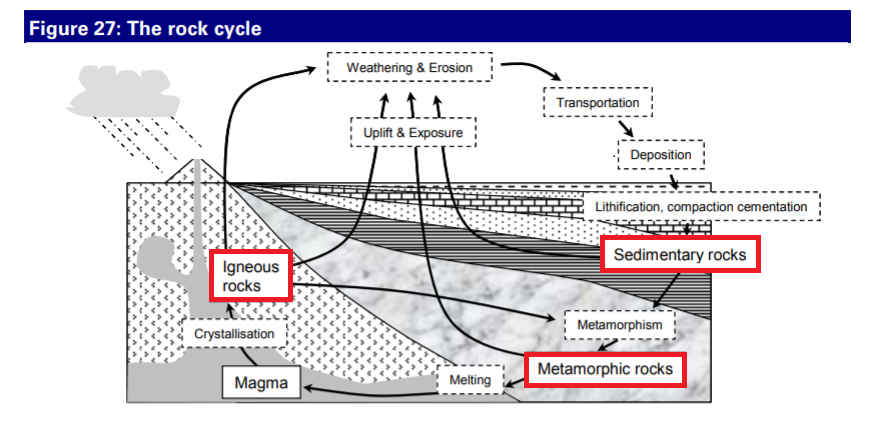
\includegraphics[width=0.9\textwidth]{figures/02-rock-cycle}
        \caption[The rock cycle]{The rock cycle describes how rocks transforms. It shows how Erosion and weather transform igneous rocks in to sedimentary rocks. Then how metamorphism transforms the latter in Metamorphic rocks. And how the crystallization of the magma of those produces igneous rocks. Adapted from the Oil and Gas beginners book \cite{oilbegin} }\label{fig:rock-cycle}
    \end{figure}

Those cycles form hydrocarbon source rocks, reservoir and seals. The movement of the plates also introduces non-linearity in the rocks where oil or gas can be trapped. Those structural traps are where we usually drill from. As we see in red on Figure~\ref{fig:rock-cycle}, there are three types of rocks: igneous, sedimentary and metamorphic. The cooling of minerals from magma  forms  igneous rocks. Metamorphic rocks are generated through  the burial process of rocks. As rocks are buried, they are exposed to higher temperature and pressure transforming organic matter into oil and gas. Sedimentary rocks accounts for almost all oil and gas reserve. They deposit in layers, reflecting the history of the depositional basin .


The hydrocarbon formation process has several steps. First the maturation where organic matter is buried and exposed to such temperature and pressure conditions that it converts into hydrocarbon.  Then follows the second part of the process: migration, it is when the hydrocarbon moves from the source rocks to the reservoir. At high temperature the oil has a lower density allowing it to move upwards through fractures in the source rocks and the reservoir rocks. At even higher temperature, the oil dissolves into gas phase. Then when it moves upwards, the pressure decreases causing it to condensate back to liquid form. The hydrocarbon is then trapped in the reservoir rock. The trap should ideally be impermeable (no fluid can flow through it). But an escape rate smaller than the production rate is sufficient for the trap to be commercially viable \cite{oilbegin}. 

Only a portion of this volume of hydrocarbon can be extracted. The amount depends on several factors such as porosity, permeability, lithology...  The following sections present some of those properties. 
\subsection{Dunham Classification}
The Duhnam classification was developed to classify carbonate sedimentary rocks. The class names describe on the depositional texture. This means that this classification is most significant for the interpretation of the depositional environment of the rocks. The Dunham classification, see Figure~\ref{fig:dunham}, follows three criteria.: the supporting fabric of the original sediment:(mud, grain ?), the presence or absence of mud, whether the original components were bound during deposition \cite{dunhamrevised}.
Those criteria lead to 4 classes :
\begin{itemize}
    \item Mudstone: mud-supported carbonate rock with less than 10\% grain.
    \item Wackestone: mud-supported carbonate rock with more than 10\% grain.
    \item Packstone: grain-supported carbonate rock with more than 1\% mud.
    \item Grainstone: grain-supported carbonate rock with less than 1\% mud.
	\begin{figure}[!htp]
    \centering
        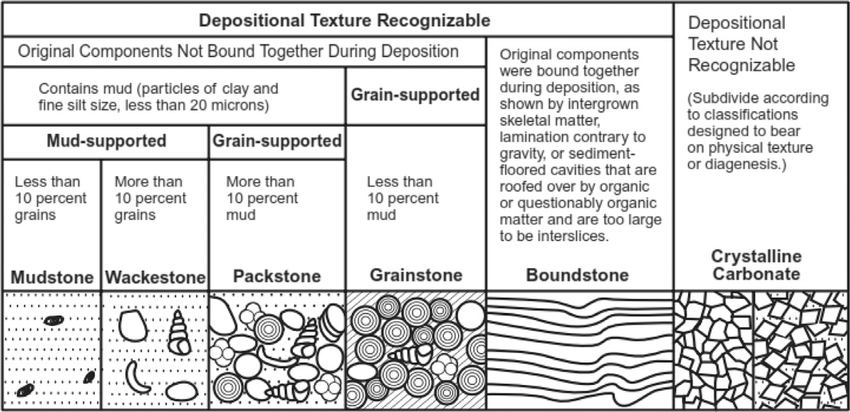
\includegraphics[width=0.9\textwidth]{figures/02-Dunhams-classification}
        \caption[Dunham Classifcation]{Dunham Classifiaction of carbonate rocks taken from Carbonate Calcium \cite{dunhamfig}}\label{fig:dunham}
    \end{figure}
\end{itemize}
This is a relevant property for reservoir rocks because it indicates what kind of rock it is: if it is going to be soft or hard to drill through...

\subsection{Porosity and permeability}

The porosity of a rock is a measure of its ability to hold fluids. This is a relevant property for reservoir rocks since it will tell how much oil they can contain. We calculate the porosity by dividing the volume of open spaces in the rock by the total volume of the rock. Porosity is expressed by a number between 0 and 1. If the porosity is 0, then the rock can't hold any fluid \cite{oilbegin}. 
 
There are two kinds of porosity:
\begin{itemize}
    \item Total porosity: it includes all void spaces regardless of whether the pores are connected or isolated.
    \item Effective porosity: it's the fraction of the total volume in which fluid effectively flows. It includes dead-ends pores but excludes non-connected pores. This is the porosity that is most relevant in petroleum studies. 
\end{itemize}

The permeability of a rock describes how easily liquid can flow through it. It is an important property for the source rocks since hydrocarbon flows through them during the migration process. But it is also important for reservoir rock since if there is low permeability, the oil contained in the pores won't be able to flow out of the rock. 
Rocks that  combine good porosity and permeability are good reservoirs . Typically, rock with high porosity and high permeability will make a good reservoir rock. Indeed, it can hold and deliver large amounts of oil. 

\subsection{Coring}\label{sec:coring}
The first step to determine where to drill is the seismic study. A big 'bang' sends wave sounds that propagates into the earth crust and are partially reflected by the different rock layers. Geophones placed on the surface gather, register and store those wave sounds. This operation is repeated several times in different places and the data gathered creates a seismic images. This images are then interpreted by geologists to identify and target zones with high chances of finding oil \cite{oilbegin}. 


Once we found an area of interest, we drill a whole is and lower sensors  to the bottom of the well to take measurements. Several instruments are used to collect those measures.  Gamma ray gives information about the level of clay, resistivity indicates potential hydrocarbon sources or sonic indicates porosity of the rock. But the best way to identify what kind of rocks we drill through is coring. This operation consists in drilling very slowly with a special drilling bit and extract a piece of the rock which looks like a tube. Then we infiltrate a resine through the core to make sure it holds and all the fragments stick together. Then we cut very thin sections out of the core, take high resolution pictures, and we ask geologist to label them. The result is a precise description of the rock the exploration is drilling through \cite{oilbegin}.  

This technique is costly since it takes days out of the normal drilling process and it can be very slow. It is also not 100\% reliable: there can be gaps in the core, it can collapse or sometimes we do not manage to extract core at all. This is why coring is not performed often. 

\section{Convolutional Neural Networks}
In the last couple of years, most of the best performing networks in image classification have been CNNs. Some of them even surpassed human accuracy for normal images \cite{humanDNN}.
A Convolutional Neural Network (CNN) is a network that makes the explicit assumption that its inputs are ordered. A rule of thumb is, if shuffling the columns of the input does not influence the results of the network, we should not use CNNs on this data. So the typiccal data used for CNNs are images and text. 
For images, the ordered aspect of the data implies that one can encode some properties into the architecture of the network. One of them is that nearby pixels are more correlated than distant pixels. This allows the network to extract local features dependant only on small sub-regions of the image and to reduce drastically the number of parameters. 


A CNN consists of three basic layers \cite{deepbook}.  In the first layer, several linear operations are performed in parallel. It produces a set of linear activation: it's the convolution layer. The second layer is the activation layer: the activation function is applied to the linear activation. This will produce a feature map representing the local features that were detected in the previous stage. The third layer is the pooling layer, this reduces the number of parameters to increase efficiency and produces a feature map. Finally, one can add a last layer: the fully connected layer, it will use the extracted features to classify the images into classes.


\subsection{Convolution Layer}

The convolution is performed on the input data by a filter or kernel to produce a feature map. We proceed to the convolution by sliding the filter over the input. The first convolution will be between the first filter and the top right part of the image. The convolution consist of a matrix multiplication and as sum which results is written on the feature map. Each filter is trained to identify a certain feature and it will detect it everywhere on the image.  Many convolutions are performed using different kernels and producing several feature map \cite{nnbook}.

Here is an example of how the feature maps are calculated. On Figure~\ref{fig:convo_calc}, the blue 3x3 matrix is the filter and the matrix on the left is the input. To get the 4 that is highlighted with green, we do a matrix multiplication followed by a sum so : 1x1 + 0x0 + 0x1 + 1x0 + 1x1 + 0x0 +1x1 + 1x0 + 1x1 = 4. 
	\begin{figure}[!htp]
    \centering
        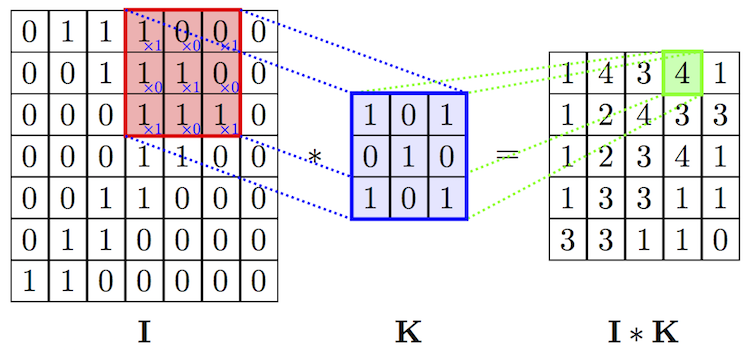
\includegraphics[width=0.9\textwidth]{figures/02-conv_layer}
        \caption[Convolution calculations]{Convolution layer calculations. The calculations are detailed above. Here the filter size is 3x3 and the stride is 1 since we are writing the 4th entry in the feature map.}\label{fig:convo_calc}
    \end{figure}
    
The area marked  in  red in the input is the receptive field. The kernel is moving over the image with a certain step size called the stride. A stride of 1 means that the kernel slides pixel by pixel. The stride length affect the size of the feature map: the larger stride length the fewer hidden neurons in the feature map. But no matter the stride size, the feature map will always be smaller than its input. This implies that if the network is deep, the feature maps might shrink. To prevent that, we use padding, which is adding a layer of zero value pixels to surround the input with. This keeps the spatial size constant after the convolution. It also improves the performance and makes sure the kernel and stride size fit with the input. 

\subsection{Pooling layer}
After a convolution layer, it is usual to add a pooling layer. The purpose of pooling is to reduce the dimensionality, the number of parameters and computations in the network. This shortens training and controls over-fitting.
The type of pooling that is mostly used is max pooling which takes the largest value in each square as shown on Figure ~\ref{fig:maxpool}. The square dimensions (2x2 on Figure ~\ref{fig:maxpool})  and the stride are determined beforehand. This layer decreases the feature map size while keeping a sufficient amount of information. 
	\begin{figure}[!htp]
    \centering
        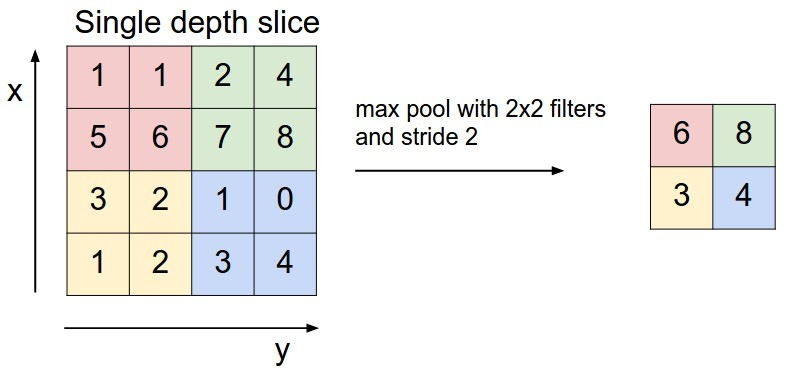
\includegraphics[width=0.9\textwidth]{figures/02-maxpool}
        \caption[Max Pooling layer]{Max pooling layer. We have a 2x2 filter with stride 2. We apply it to the output of the previous layer and it takes the maximum value of each 2x2 window. Taken from the Stanford course on CNNs \cite{cs231n}}\label{fig:maxpool}
    \end{figure}
 
   
Most of the pooled output values have very small transitional variance. This means that a translation in the input won't impact the output too much. This is very valuable since it is more important to detect the feature than to know precisely where it is situated in the image. The max-pooling will forget the exact position to focus on the relative position compared to the other features \cite{cs231n}.

\subsection{Classification Layer}
\label{sec:class_lay}
After the pooling layer, most CNN architecture will have one or more fully connected layers. Those layers are connected to all the input neurons. To perform the classification, we need this fully connected layer to have as many output neurons as classes to classify. So if you are trying to classify between red and white for example, you would have two output neurons.  It also needs to be combined with an activation function. This way, it outputs a probability distribution that allows the network to predict the class that has the highest probability. The choice of the activation function depends on the nature of the classification task \cite{deepbook}.
\subsubsection{Single label classification}
When a network is trying to predict only one class, we usually use a softmax activation function. It is defines as follows: \[softmax_j(x) = \frac{e^x_j}{\sum\nolimits_{k} e^x_k} \]Softmax is useful because it converts the output of the last layer in the network into normalized class probabilities. So the probabilities sums up to one. It makes it easy to identify the most likely output since it will be the one with the highest probability. 
\subsubsection{Multi-label classification}
The specific property of softmax that makes the probability sum up to 1 makes it unusable for multi-label classifications. Which is when one picture can have several labels. So for that case, we use the sigmoid function as activation for the last layer. It will produce values between 0 and 1. The high values of output will be interpreted as high probability. We can chose a threshold for label selection, for example 0.5. We then say that if the value for the output of the sigmoid is greater than 0.5, we predict the label, otherwise we don't. This allows several labels to be predicted since more than one label can have a high value. 

\section{Optimization}
The aim of the training and optimization process is to tune the networks parameters in order to predict efficiently labels. To do that, we need to define an objective function which value measures the error between the prediction and the label. During the optimization, we use several methods to adjust the parameters to minimize the objective function.

\subsection{Losses}
%%Editing note: (REF : \url{https://ml-cheatsheet.readthedocs.io/en/latest/loss_functions.htm}l)
We use two different objective functions in this thesis. The cross-entropy for single label classification and the binary cross entropy for multi-label classification. We will also refer to it as the loss. 
For single label classification, we define the cross-entropy loss as follows: \[H_y'(y) = - \sum\nolimits_k y'_k log(y_k)\] Where \(y_k\) is the predicted probability for class k and \(y'_k\) is the true probability for this class. It measures the performance of a classification which outputs probabilities between 0 and 1. On  Figure~\ref{fig:CE} , we can see that the closer we get to the true label, the smaller the loss. But when the probability decreases, the loss increases very quickly. So prediction that are very confident but wrong are more penalized \cite{nnbook}.
\begin{figure}[!htp]
    \centering
        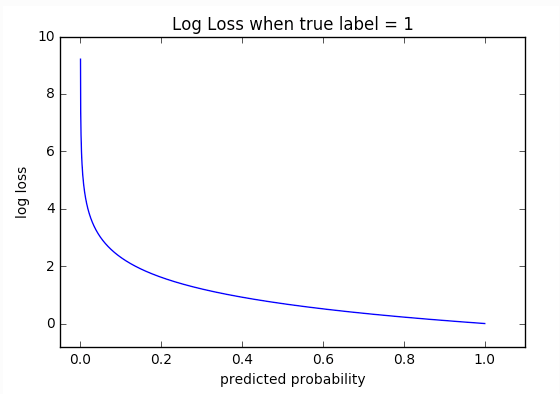
\includegraphics[width=0.7\textwidth]{figures/02-cross_entropy}
        \caption[Cross Entropy loss behaviour]{Cross Entropy loss behaviour. When we get close to the good prediction, the loss decreases slowly. But when we get further, the loss increases quickly. Plot taken from \cite{celoss}}
        \label{fig:CE}
\end{figure}


For multi-label classification, we use the binary cross entropy loss. That is because we are not treating our labels as integers, but their one hot encoded representation. For single-labels, if we have three classes, label for class 1 will be 1, label for class 2 will be 2 etc...  For multi-label, we need to have the ability of having more than one label. A label for class 1 will then be [1, 0, 0], label for class 2 [0, 1, 0] and if an item is in class 1 and 2 its label will be [ 1, 1, 0]. So in the case the values of \(y'_k\) are 0 or 1, we use binary cross entropy loss which is defined as follows: \[H_y'(y) = - \sum\nolimits_k y'_k log(y_k)\ + (1 - y'_k)log(1 - y_k) \]

Those are basically two different formulation of the same loss. They have the same behavior and can both be referred to as log loss. 
\subsection{Gradient Descent and Learning rate}
%% Editing note: . LEX FRIDMAN MIT
%% Editing note: RF : https://towardsdatascience.com/gradient-descent-in-a-nutshell-eaf8c18212f0
 "A gradient measures how much the output of a function changes if you change the input a little bit", Lex Fridman, MIT. 


In order to minimize the objective function, we use gradient based methods. The gradient descent is an iterative method which updates the parameters of the network with the aim of minimizing the objective function. By moving the parameters in a small step in the opposite direction of the gradient, we reduce the objective function \cite{cs231n}. 

Let J(\(\theta\)) be our objective function and \(\theta\) the parameters of the network. The gradient descent updates the parameters as follow: \[\theta' = \theta - \eta . \nabla_\theta J(\theta) \] The learning rate \(\eta\) determines the impact of these updates on the parameters. \(\nabla_\theta J(\theta) \) is the gradient of the objective function. At every iteration, the objective function is one step closer to the local minimum. The size of this step is influenced by the learning rate, but also by the objective function itself: a big loss will result in big updates. 


The learning rate plays a crucial role: if it is too high, the learning might miss the local minimum and if it's too small, learning might be very slow. In both cases the biggest risk is that our function never converges to its local minimum. Either because it keeps bumping on the gradients convex function or because it takes too long, see Figure~\ref{fig:LR}  \cite{cs231n}.  
\begin{figure}[!htp]
    \centering
        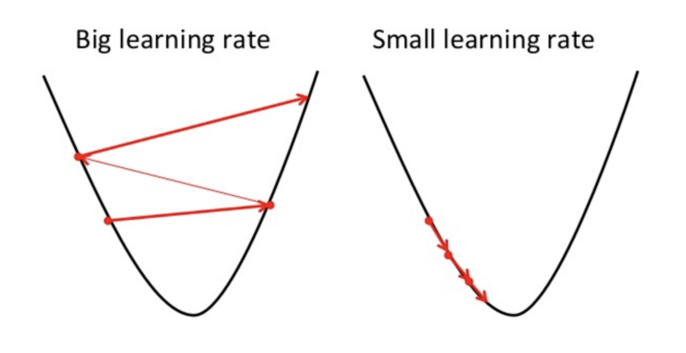
\includegraphics[width=0.9\textwidth]{figures/02-LR}
        \caption[Gradient behaviour for different learning rates]{Gradient behaviour for different learning rates. On the left, the learning rate is too big so the gradient bounces back and forth on the function. On the right it is too small so it converges very slowly towards the minimum. Figures taken from \cite{gradient} }\label{fig:LR}
\end{figure}

The Figure~\ref{fig:LR_impact} shows the different behaviours of the training loss based on the value of the learning rate. The yellow curve shows a very high learning rate. The loss explodes quickly, the gradient has taken such a big step that it most likely exited the local minimum and it can't converge. The green curve shows a bit smaller learning rate. The gradient goes down the curve but then bounces back and forth on the gradient curve as on Figure~\ref{fig:LR}. It will converge to a non optimal value of the loss. Then the blue curve shows a way to small learning rate. The gradient updates the weight too slowly and they are not corrected enough to reach the optimal loss value in time. Finally the red curve shows a good learning rate. Early in the training, we take big steps in the gradient so the loss decreases quickly. But when we are close to the local minimum, the steps are smaller and the loss converges \cite{lr}. 

%% Editing note :  RF :https://towardsdatascience.com/understanding-learning-rates-and-how-it-improves-performance-in-deep-learning-d0d4059c1c10
There are different strategies to chose the good learning rate. A good general idea is to start with a big learning rate to learn quickly in the beginning and make it smaller as we go along with the training. 
\begin{figure}[!htp]
    \centering
        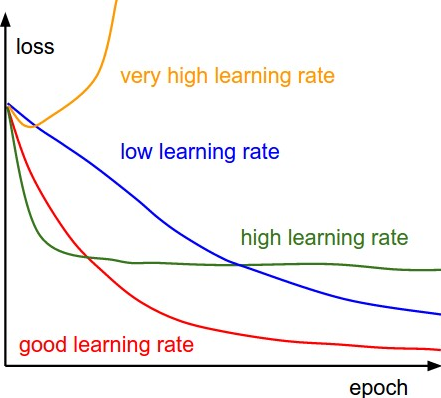
\includegraphics[width=0.5\textwidth]{figures/02-LR_impatc_train}
        \caption[Impact of the learning rate on training]{Training loss evolution based on different values of the learning rate. This image has been taken from \cite{cs231n}}\label{fig:LR_impact}
\end{figure}

\subsubsection{Gradient Descent variant}
There are three variants of gradient descent which differ in the amount of data we use to compute the gradient of the cost function \cite{gradient}. 
\begin{itemize}
    \item The batch gradient descent compute the gradient of the cost function for the entire training dataset. This is computationally efficient and gives a stable error gradient but it is intractable if the dataset does not fit in memory. 
    \item The second variant is stochastic gradient descent which computes the gradient for every training example. It can be redundant since we recompute the gradient for very similar training examples.
    \item The third variant is a compromise between the two others, it computes the gradient for every mini batch of n training example. This reduces the variance of the parameter update without wasting computation. It can also lead to a more stable convergence.
\end{itemize}There are still challenges, mainly regarding the learning rate. As we stated earlier, it is difficult to find a good value for it. A solution is to reduce the learning rate according to a specific time line. We can divided it by 10 every ten epoch for example, or when the cost function is below a fixed threshold. This works well but they have to be defined in advance so they don't adapt to the data. The ultimate challenge is to keep the gradient from getting stuck in local minima or saddle points. Some algorithms or additional parameters have been implemented to overcome those challenges
\subsubsection{Momentum}
Around a local minimum, the surface curves are often steeper in one dimension than the others, this is called a ravine. In those areas, the gradient descent oscillates across the slopes and converges slowly to the local minimum. The momentum helps to achieve convergence faster by speeding up the gradient descent in the good direction. For that, it remembers the value of the update vector at the past iteration and uses it to calculate the new update \cite{optimgrad}. \[ v_t = \gamma v_{t-1} + \eta . \nabla_\theta J(\theta)  \] \[\theta' = \theta - v_t\]
Where \(v\) is the velocity and \(\gamma\) is the momentum term. The velocity represents the direction and the speed of the parameters. \(\gamma\) determines how much the velocity term impacts the update. With momentum, the gradient keeps in memory the direction the gradient was going before. So if the gradient keeps going in the same direction, it will gain velocity and make bigger updates. But if there is a brutal change of direction, the update will be moderated and there will be less oscillations. A common analogy for this is to imagine a ball going down a hill. While it rolls down, the momentum adds mass, making it go faster and overcoming smaller bumps \cite{optimgrad}. A risk of this technique is that if the gradient accumulates too much velocity in one direction, it might overlook a local minimum. 

\subsubsection{Adam Optimizer}

An other optimization algorithm is ADAM and stands for Adaptive Moment Estimation. It computes adaptive learning rates for each parameter . Adam stores estimates of the first and second moments - \(m_t\) and \(v_t\) - which are respectively the mean and the uncentered variance of the gradient. They are computed as follow: \[ v_t = \beta_2 v_{t-1} + (1 - \beta_2)g_t^2 \] \[m_t = \beta_1 m_{t-1} + (1 - \beta_1)g_t \]
Where \(\beta_1\) and \(\beta_2\) are the learning rates and \(g_t\) is the gradient. The parameter are updated taking into account both, how much the gradients are changing on average but also from one iteration to the other.  \(m_t\) and \(v_t\) are initialized as 0 vectors. Experiments shows that they are biased towards 0, especially during the early steps are when the learning rates are small. We handle this bias by producing estimates of the first and second moment that are bias corrected \cite{adam}. \(\hat{m}_t\) and \(\hat{v}_t\). 
\[ \hat{v}_t=  \frac{v_{t}}{1 - \beta_2^t}\] 
\[\hat{m}_t=  \frac{m_{t}}{1 - \beta_1^t}\] 
We then use those estimates to calculate the parameters update as follow: \[\theta_{t+1} = \theta_t - \frac{\eta}{\sqrt{\hat{v}_t} + \epsilon}\hat{m}_t\]
Where \(\eta\) is the general learning rate for the parameter update and \(\epsilon\) is a small constant to ensure mathematical stability. 
The detailed  Adam algorithm is presented in Algorithm \ref{fig:adam_algo}.
\begin{figure}[!htp]
    \centering
        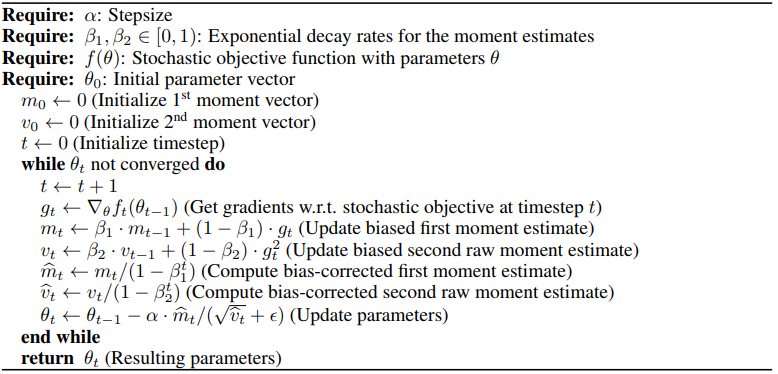
\includegraphics[width=0.5\textwidth]{figures/02-adam_algo}
        \caption[Adam Algorithm]{ This Algorithm is a optimization of the stochastic gradient descent. It describes the update rule for the first and second moment. Algorithm of has been taken from \cite{adam}}\label{fig:adam_algo}
\end{figure}
The Adam optimizer is an iterative algorithm. It means that the parameters will be updated until they reach the stopping criterion. 
Adam optimizer has shown that it achieves good results fast and is thus used as a default in many 
computer vision and deep learning algorithms. Several variants exists.

\subsubsection{Adamax}
One variant of the Adam algorithm is the Adamax optimizer. In the Adam algorithm. we use the \(L^2\) norm to update \(v_t\). This can be generalized to a \(L^p\) norm based update rule that would write as follows : \[ v_t = \beta_2^p v_{t-1} + (1 - \beta_2^p) \mid g_t\mid^p \] . This variant will become unstable as p gets bigger than 1 or 2. Surprisingly, as \(p\to\infty\), the behavior is simple and stable. If we then defined \(u_t\) as \[u_t = \lim_{p\to\infty}(v_t)^{1/p}\]
\[u_t = \lim_{p\to\infty}(\beta_2^p v_{t-1} + (1 - \beta_2^p)\mid g_t\mid^p)^{1/p}\] 
\[u_t = \lim_{p\to\infty}(1 - \beta_2^p)^{1/p}(\sum_{i=1}^{t}\beta_2^{t-i} \mid g_i\mid ^p)^{1/p}\]
\[u_t = \lim_{p\to\infty}((1 - \beta_2^p) \sum_{i=1}^{t}\beta_2^{t-i} \mid g_i\mid ^p)^{1/p}\]
\[u_t = \lim_{p\to\infty}(\sum_{i=1}^{t}\beta_2^{t-i} \mid g_i\mid ^p)^{1/p}\]
\[u_t = \max (\beta_2^{t-1}  \mid g_1\mid, \beta_2^{t-2}  \mid g_2\mid ), ..., \beta_2^ \mid g_{t-1}\mid, \mid g_t\mid\]

The last equation can be very easily written recursively: 
\[ u_t = \max(\beta_2 . u_{t-1},  \mid g_t\mid)\]
As shown on Algorithm \ref{fig:adamax_algo}, \(u_t\) is initialized to 0 and then plugged in the Adam update: 
\[\theta_{t+1} = \theta_t - \frac{\eta}{u_t} \hat{m}_t\]

\begin{figure}[!htp]
    \centering
        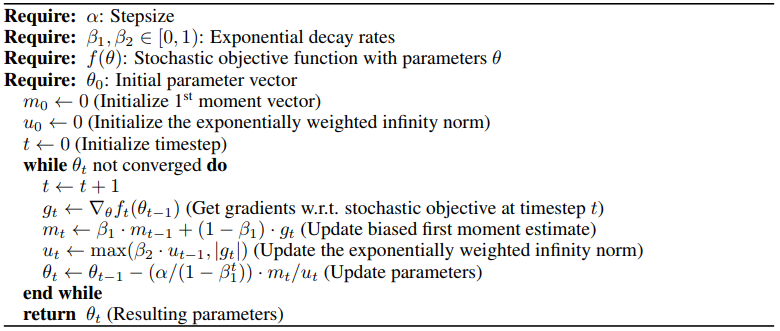
\includegraphics[width=0.9\textwidth]{figures/02-adamax_algo}
        \caption[Adamax Algorithm]{ This Algorithm is a variant from the Adam algorithm presented below. It is based on the infinity norm. The proof of why we use the max operation is explained in this section. Algorithm of has been taken from \cite{adam}}\label{fig:adamax_algo}
\end{figure}

As \(u_t\) relies on the \(\max\) operation, it does not have a bias towards 0. This is why we do not need to calculate an estimate nor add a stabilization constant as for \(\hat{v}_t\) to calculate the update rule \cite{adam}.

\section{Accuracy and Validation metrics}
In order to find out how a model is performing, we need to chose some metrics. The most popular one is accuracy since it speaks to anyone even not familiar with the field. But it can be limited in some cases and give a false impression that the model is doing well when it actually isn't. To get a better overview, we use precision and recall. 

\subsection{F1 score}
While accuracy is a good indication of how well the model is performing, they can give erroneous information. Let's say you are trying to identify people with a rare disease. You could very easily produce a model with 99.999999\% accuracy to identify a sick person simply by labeling every single individual as sick. So you produces a model with a nearly perfect accuracy, but with no value. In cases where there is quit a big imbalance between classes, the accuracy won't be a good measure of performance.
What is important in our toy case is to identify as many of the relevant cases as possible, this is similar to maximizing the recall \cite{multimetrics}. 

Recall calculation uses true positive (samples classified as positive that are actually positive) and true negatives (samples classified as negative that are actually positive). The recall is then defined as the number of true positives divided by the sum of the true positives and false negatives \cite{metrics}. 


\[recall = \frac{True Positives}{True Positives + False Negatives} = \frac{Sick People Correctly Identified}{Actually Sick People}\]
But a model with very high recall will have a bad precision. We would not want to tell healthy people that they are sick. 

The precision focuses on the proportion of samples we said were correctly classified actually were. For that we introduce false positives (samples classified as positive that are actually negative). The precision is then defined as the number of true positives divided by the sum of true and false positives \cite{metrics}.
\[precision = \frac{True Positives}{True Positives + False Positives} = \frac{Sick People Correctly Identified}{People Identified As Sick}\]
 In cases where we want to find an optimal trade-off between precision and recall, we use the F1-score which is defined as 
 \[F1 = 2*\frac{precision * recall}{precision + recall} \]
 The precision is a measure of a classifier's exactness while recall is a measure of a its completeness. 
 We use a harmonic mean to avoid giving good F1 scores to models with extreme values: 1 of recall and 0 of precision for example \cite{wiki-f1}. 
In some cases, samples can have more than one labels, and the different classes can be unbalanced. A way to handle that is to calculate the F1 score by calculating it for each class.  Then we do a weighted sum to take into account class that are more populated than others. 
There are several ways to visualize precision and recall, one of the prettiest way is to use confusion matrices. 
\subsection{Confusion Matrix}

\begin{figure}[h]
    \centering
        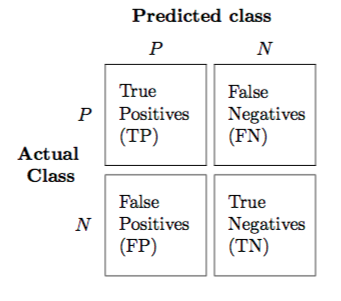
\includegraphics[width=0.5\textwidth]{figures/02-CM}
        \caption[Confusion matrix]{Confusion matrix for a binary classification. This is a good way to rapidly visualize true positives, false negatives... And it is also easy to calculate precision and recall. Figure taken from \cite{cm_image}}\label{fig:CM}
\end{figure}

A confusion matrix is a an overview of the precision and recall results of a classification problem. The columns represent the number of occurrences of the predicted labels for each class. The rows represent the count of occurrences of the real labels for each class. It shows how the classification task is confused. This gives insight on the kind of error being made \cite{cm}. 

It is relevant to know if your model is more likely to mix up  a German shepherd for a fox or a fox for a turtle! It makes the interpretation of the results better since you know how your model is biased. Also, some errors are more acceptable than others. One can consider a model with lower accuracy but miscalssifying similar objects better than a model with very high accuracy but missing simple cases. 
It makes it also easy to get the precision and the recall of the model. On Figure~\ref{fig:CM}, we see clearly how to identify true and false positives and negatives. This makes the calculation that we saw in last section easy to make. 



\section{State of the art networks}
Image classification is a challenging task that needs to more complex CNNs. I focus on three network architectures that have proven to give significant results in the classification task. Today, ResNet is the one that achieves the best results and AlexNet is the one that does it in the shortest time.    

\subsection{GoogLeNet and Inception-v3}
GoogLeNet was the winner of the ILSRVC in 2014, it also known as Inception V1. It is a CNN inspired by LeNet that introduces a new type of module called inception. Those modules can bee seen as smaller models within the network. 

In classic architecture, you have to decide at each layer which size the filters for the convolution should be: 5x5, 3x3... But from one image to another, the location of the information and its size can vary a lot. That is why it is difficult to know beforehand which of those convolutions would give the best result. The inception module tackles this problem by performing all the convolutions in parallel. It then concatenates the different feature maps before passing it on to the following layer. This way, the model can pick up both local features from the small convolutions and more general features with bigger convolutions \cite{googlepaper}. 

Figure~\ref{fig:inception} shows the detailed implementation of the inception module. As we explained before, 1x1, 3x3 and 5x5 convolutions are done in parallel. The max-pooling layer is added because it has been successfully used in most current state of the art networks. Also a 1x1 convolution as well as a ReLu activation are added to reduce the dimensionality of the feature map. This way we reduce the number of parameters before passing it to the bigger convolutions. The GoogLeNet is 22 layers deep and stacks convolution layers and inception module as presented in Figure~\ref{fig:googl}

\begin{figure}
\begin{subfigure}{.5\textwidth}
  \centering
  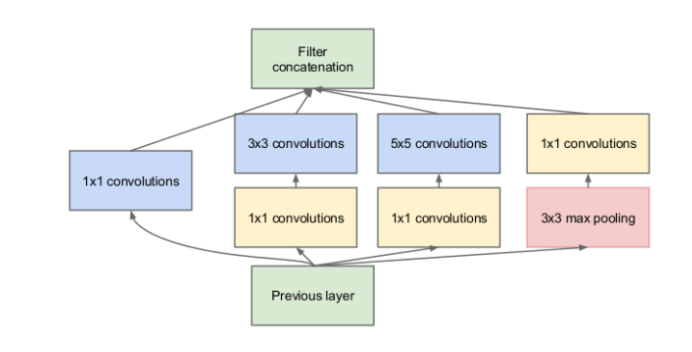
\includegraphics[width=.8\linewidth]{figures/02-inception_module}
  \caption{The inception module with dimensionality reduction }
  \label{fig:inception}
\end{subfigure}%
\begin{subfigure}{.5\textwidth}
  \centering
  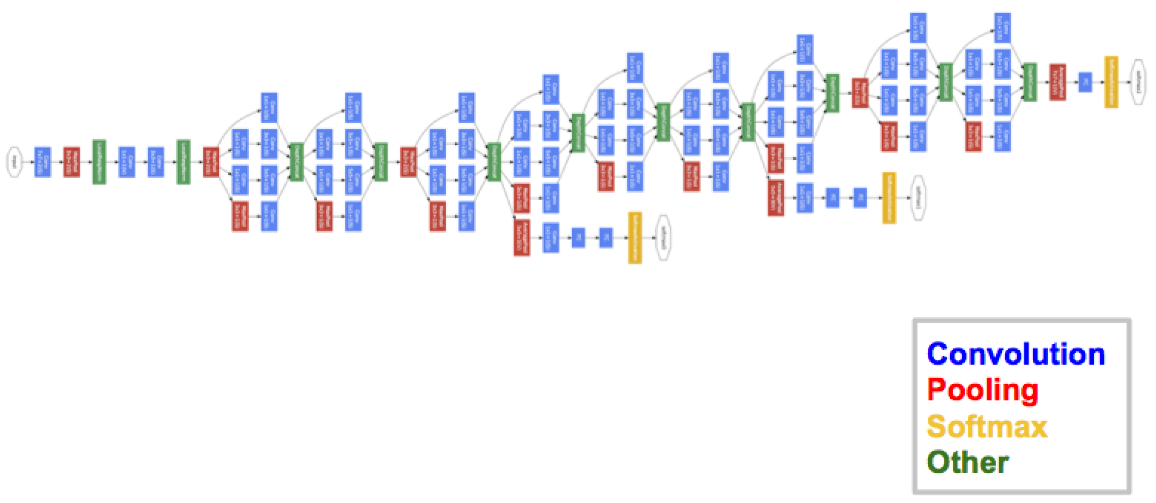
\includegraphics[width=.8\linewidth]{figures/02-googlearch}
  \caption{Full 22-layers architecture of GoogLeNet}
  \label{fig:googl}
\end{subfigure}
\caption[Inception network architecture]{Detailed and overview of the architecture of GoogLeNet. Both images have been taken from the original paper \cite{googlepaper}}
\end{figure}
Some optimization were presented in (going deeper paper). The first one is Inception-v2 which tackles the issue of representational bottleneck. This happens when one use reduces the dimension of the input too much resulting in a loss of information. It solves this issue by replacing the 5x5 convolution by two 3x3 convolutions, which also boosts the performance. On top of that Inception-v3 implements a RSMSProp optimizer,. It also performs a factorization of the 7x7 convolutions in a similar way as Inception-v2 and label smoothing. 

\subsection{ResNet}
ResNet won first place in the ILSRVC 2015 image classification competition. It introduces a new network architecture called Residual Learning. 

When deep networks get even deeper, the accuracy gets saturated and decreases rapidly: this is the degradation problem \cite{resnetpaper}. That is the issue Residual Learning aims at solving. This phenomenon is surprising since one would think that a network with extra layers would learn as much, if not more, than a shallower network. But experiments prove that this is not the case. Deeper networks gets a worse accuracy than shallower ones, see on the left of Figure~\ref{fig:resnetaccs}. The 34-layers plain network has a higher error than the 18-layers network. 

\begin{figure}[!htp]
    \centering
        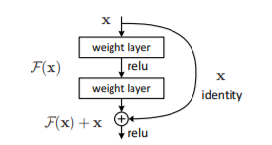
\includegraphics[width=0.9\textwidth]{figures/02-resnet_block}
        \caption[Building block of Resnet]{Building block of ResNet. Instead of having only stacked layers, we also have the identity function. Figure taken from the original paper \cite{resnetpaper}}\label{fig:resnetblock}
\end{figure}
%% Editing note : medium article 
A regular network architecture learns the mapping of input x to output y with a function H(x) which is a few stacked non linear layers. ResNet architecture defines a residual function using F(x) = H(x) – x which can be expressed as F(x) = H(x) + x. H(x) is a few stacked non linear layers and x is the identity function, see Figure~\ref{fig:resnetblock}. The intuition behind this architecture is that if the identity mapping is optimal (we want the input to be equal to the output), it’s easier to drive H(x) to 0 and only keep the identity than to fit H(x) to the identity \cite{mediumresnet}. In practice, identity mappings are rarely optimal. But the hypothesis that it’s easier to optimize a residual mapping  than the original mapping is proven during experiments. Figure~\ref{fig:resnetaccs} shows that ResNet overcomes the degradation problem. It also achieves better results than its plains counterparts.


\begin{figure}[!htp]
    \centering
        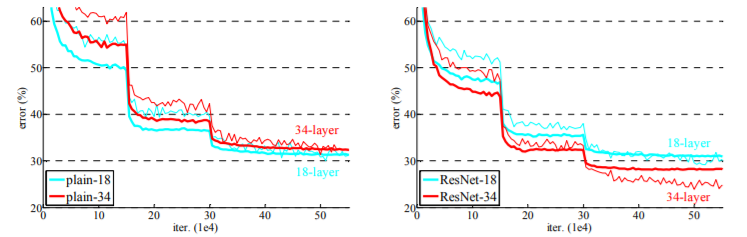
\includegraphics[width=0.9\textwidth]{figures/02-Resnet_comparing_acc}
        \caption[Degradation problem solved]{Training on ImageNet. Thin curves are training error, and bold curves are validation error of the center crops. Left: plain
networks of 18 and 34 layers. Right: ResNet of 18 and 34 layers. Taken from the riginal paper \cite{resnetpaper}}\label{fig:resnetaccs}
\end{figure}

\subsection{AlexNet}
AlexNet architecture focuses on parallelizing CNNs across multiple GPUs. It won first place in the ILSRVC in 2012. It had a great impact on deep learning and computer vision since it allowed networks to scale better than all alternatives.
The idea is to parallelize in different ways depending on the kind of layer the network is training\cite{alexpaper}. There are two ways of parallelize the training of a network : 
\begin{itemize}
    \item Model parallelism: different workers train different parts of the model. The workers must synchronize whenever a model part trained by a worker needs output from another model part trained by an other worker.  
    \item Data parallelism: different workers train on different data samples. The workers must synchronize the model parameters to make sure they are learning a consistent model. 
\end{itemize}
As we saw in section 2.3, CNNs consist of two types of layers. Convolutional layers that contain most of the computations (between 90 and 95\%) and fully connected layers that contains most of the model parameters (around 95\%). In AlexNet, the convolutional layers rely on data parallelism while fully connected layers rely on model parallelism \cite{alexpaper}. 

This is illustrated on Figure~\ref{fig:alexnet}. 
\begin{figure}[!htp]
    \centering
        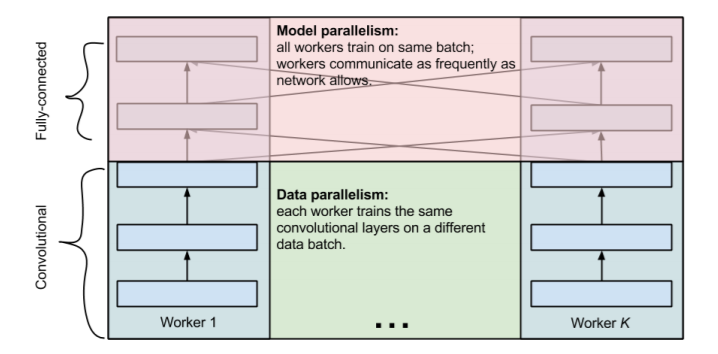
\includegraphics[width=0.9\textwidth]{figures/02-alexnet}
        \caption[AlexNet architecure overview]{Training of a network with 3 convolutional layers and 2 fully-connected layers by K workers. Taken from the original paper \cite{alexpaper}}\label{fig:alexnet}
\end{figure}
What happens is that each of the K workers is given different data batch and computes all the convolutions on its data: this is data parallelism. Then it switches to model parallelism. One worker sends its last staged convolution to all other workers.  Then it computes the fully-connected layers and start back propagation. In parallel, the next worker sends its last-stage convolution to all other workers. They can then compute the fully-connected layers on the second batch and so on. The same behavior is implemented in the back propagation. 

\subsection{Transfer Learning} \label{sec:translearn}
%% Editing note \url{https://arxiv.org/abs/1411.1792} 
%% Editing note: . \url{https://ieeexplore.ieee.org/stamp/stamp.jsp?arnumber=5288526}
%% Editing note: link to c231n course)
There are few database big enough to properly train those networks. And when there is, it can takes weeks before the network achieves acceptable results. A more clever way to use those networks is through transfer learning. This technique relies on the fact that what a network learns from a data set is still useful for another data set \cite{translearnsurvey}. To transfer this knowledge,  we download the weights used to achieve the best performance of a network on an sufficiently big data set. Then we build our training algorithm on top of that network. A very important property underlying this is that the deeper the layers of a network, the more complex shapes the network learns \cite{layerslearn}. So the early layers learn the basic shapes, colors... while deeper layers learn complex shape, and more subtle variation in the image. 
There are two major ways of using transfer learning. 
\begin{itemize}
    \item Fine-tuning: The network is initialized - all the parameters of every layer - with the pretrained network. The network is in most case pretrained on the ImageNet data set on 1000 classes. It is just another way to initialize weights, nothing is changed further in the training algorithm \cite{cs231n}.
    \item Network acts as feature extractor: An other way to use it is to set all the weights to the pretrained ones. Then freeze them all, except the ones in the final fully connected layer. This last layer is initialized to random weights and only those weights are modified during the training. 
    This technique is quicker since gradients are only computed for the last layer
\end{itemize}
Those two techniques can be adapted.  An alternative would then be to freeze the k first layers and just learn again the n-k remaining ones to adapt it best to our classification task. For example, if the classification problem contains images that are very different to the ones contained in the ImageNet, we might want to retrain most of the model \cite{translearnsurvey}. 
Using transfer learning helps achieving faster and better results. Since it starts from a very advanced level instead of starting from 0, the networks converges and learns much more quickly on the new data.

\section{Data Augmentation} \label{sec:dataug}
As mentioned in the section above, it is rare to find data sets big enough to train the state of the art networks. Some tricks exists to make your data set bigger. It is called data augmentation. The aim is to create more training data from the ones that we already collected. The most common operations are rotations, flips, resizing, rescaling etc... Other techniques that changes the image a bit more can also be used.
\begin{itemize}
    \item Color Jitter: It is a gentle way to change the brightness, contrast, hue and saturation of the image. 
    For each parameter p, Color Jitter chooses a random value v between 1 - p and 1 + p and then applies the parameter adjustment with this value v. So for example, if we chose to set the brightness parameter to 0.3. The method will chooses a random value between 0.7 and 1.3, let's say 1.05 and adjust the brightness with a intensity of 1.05. This is why it is important to keep the values small. Indeed, if we chose 0.8 for brightness for example, we risk to have it adjusted with an intensity of 0.2 which would result in an almost completely black image.
     \item Elastic Transform:   Elastic transformation rely on the fact  that images have some invariance to elastic deformation. Elastic deformation describes the temporary deformation of a material that will later regain its original form. Instead of moving the whole image as in affine transformation, we move each pixel to a new position dependent of the previous one \cite{elastic}. This can be seen as a grid underlying the image. Each point of the grid will be slightly moved, resulting in a distorted image. 
     \end{itemize}
\chapter{Methodology}\label{chp:methodology}
In this chapter we explain the research methods used and rationalize their choice. Further, we present the pre processing and label selection, the detailed architecture of the networks and the different experiments that have been conducted. 
\section{Data}

As explained in Section~\ref{sec:coring}, the data has been gathered through coring and labelled by geologists. Further on, we will consider the geologists labels as the ground truth. We have gathered 1907 labeled images. 

\subsection{Label Selection}
 The labels of every image can be divided into different classes, see Figure~\ref{fig:classes}. For example, the class Lithology contains 10 different labels, each representing one of the possible lithologies. Not all images have labels in every classes, that is why some classes are under-represented. The classes Dominant Grain type, Diagenesis, Cutting description and Sorting have less than 1000 data points. This is not enough to produce good prediction, that is why we chose not to use them.
 
 For the classes that are sufficiently populated, we plot the distribution of the data points within those classes. In Figure~\ref{fig:litandstruct}, we can see the labels distribution for Lithology and Structures. The labels are extremely unbalanced, so trying to predict any other label than Lit1 for Lithology and Structure 1 or 2 for Structures would be very difficult. This is why we will not try to predict on those class. 
 The remaining classes : Porosity, Components, Dunham and DRT, have a good distribution of points within the class. They also give a good overview of the rock properties. If we are able to predict correctly on them, we will have an idea of how good the reservoir rock is. 
\begin{figure}
\begin{subfigure}{1\textwidth}
  \centering
  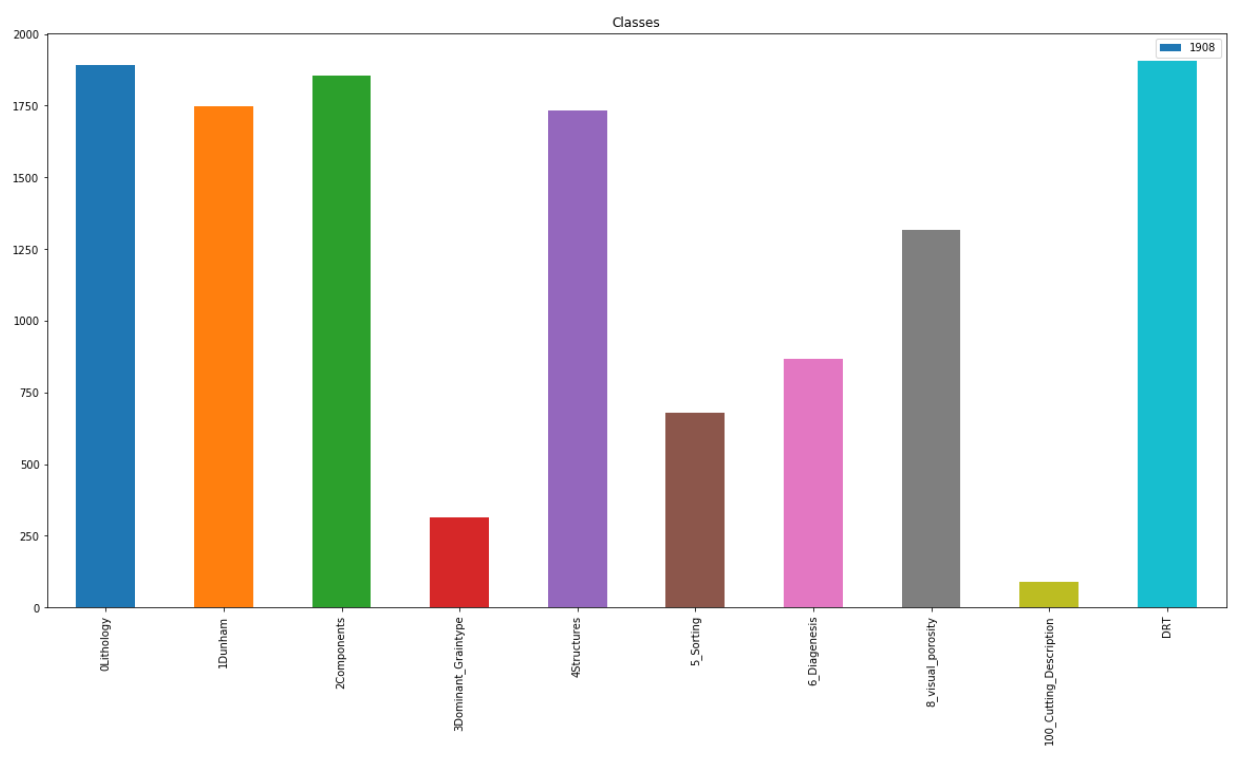
\includegraphics[width=.8\linewidth]{figures/03-classes.png}
  \caption{Classes over the samples}
  \label{fig:classes}
\end{subfigure}%
\\
\begin{subfigure}{1\textwidth}
  \centering
  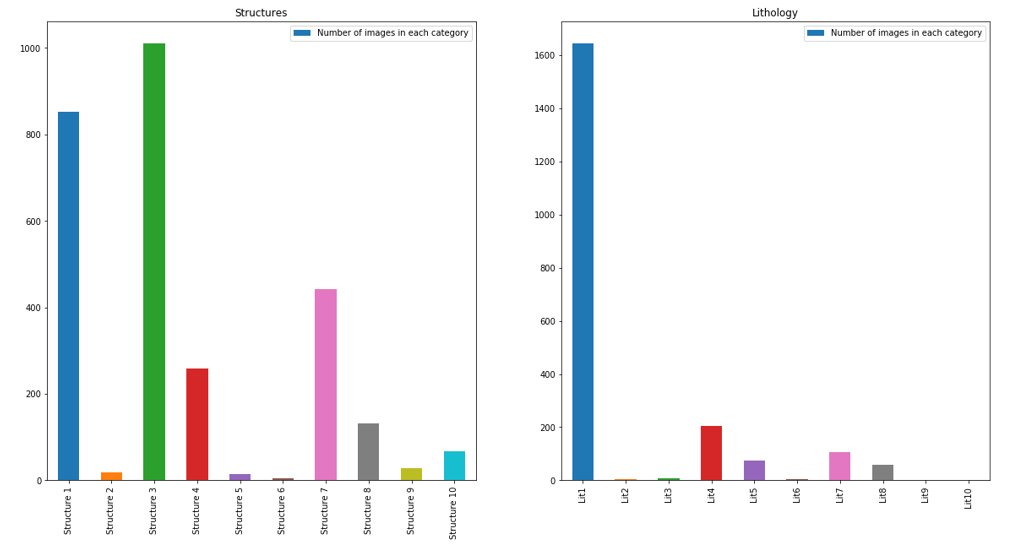
\includegraphics[width=.8\linewidth]{figures/03-boob.PNG}
  \caption{Lithology and Structure over samples}
  \label{fig:litandstruct}
\end{subfigure}
\caption[Classes distributions]{Distribution of different classes over the whole data set.}
\end{figure}


\subsection{Label pre-processing}
Once we selected the four labels to predict on, we looked into the details of the distribution and adapted it to make it easier to predict on. For the Dunham labels, the first class was under represented, only seven samples. So we decided to simply cut it out. We now have six classes that are almost homogeneously distributed, see Figure~\ref{fig:dunham}. 

For the porosity labels, there are two different levels of description of the porosity. The first level is the amount of porosity: no, minor, intermediate or abundant. The second is the kind of porosity: patchy or micro-porosity. In a first pass, we will only focus on the quantitative aspect: how much porosity do we observe in each sample, see Figure~\ref{fig:porolab}. A further analysis would be to determine what kind of porosity accounts for this total porosity. It might be considered at a later stage. Also, for this first experiment, after we have extracted four labels, we sorted them from no to abundant porosity. 

As shown in Figure~\ref{fig:drtlab} and Figure~\ref{fig:compolab}, the DRT and components class have a lot of different labels: 19 and 13 respectively. Some of them are not populated enough to be considered. Some of the labels we chose to keep are still under-represented but we believe they are populated enough to be predicted.

We can divide the classes into two main categories. The DRT and Dunham labels are single-label multi-class labels. It means that each image can only have one label within a class. The Components label are multi-labels multi-class labels, meaning that one image can have one or more label. The porosity has two levels of labels, so we can consider porosity as being both single-label (if we only look at the amount) or multi-label labels. 


As we can see in Figures~\ref{fig:dunhamlab} to ~\ref{fig:compolab}, our labels are not equally distributed. Thus, the network will be biased towards the most populated labels. A way to counter this would be to get more samples of the under represented class. But when one is trying to characterize a certain geographical area, it is normal to find rocks and components that are more present than others. We deal with this issue by calculating the loss with weights. We want to teach our model to give a higher weight to a sample with an under represented label, than one with a more represented label . This way, it should not favor most populated class. 

For single label classification, we calculate the weights of each class as follows: weight of class A is the total number of samples divided by the number of samples in class A.

For multi-label classification, the labels are represented as one-hot encoded vectors as we saw in section~\ref{sec:loss}. We calculate the weights as follows: weight of class A is the number of 0 in class A divided by the number of 1 in class A.

\begin{figure}
\begin{subfigure}{.6\textwidth}
  \centering
  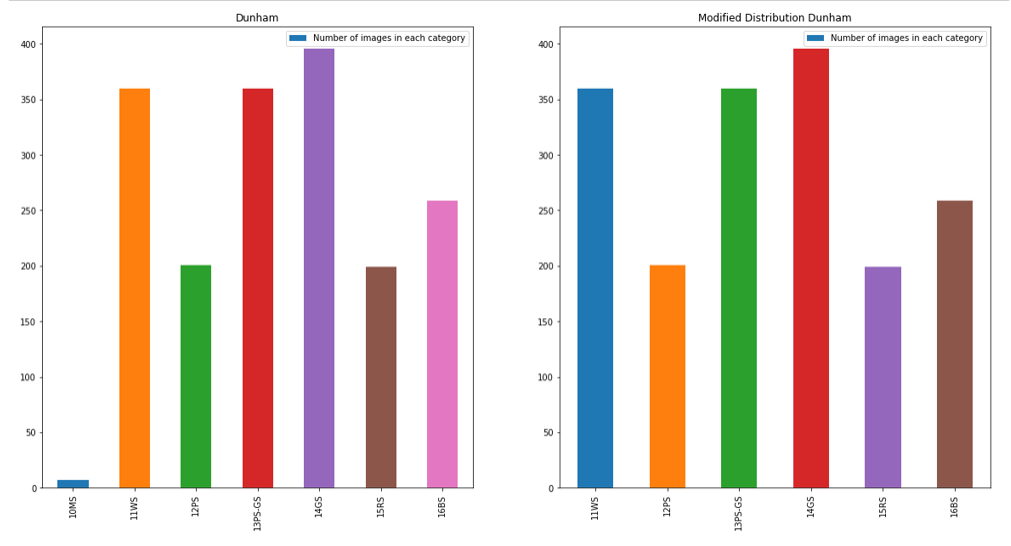
\includegraphics[width=1\linewidth]{figures/03-Dunham.PNG}
  \caption{Dunham Labels}
  \label{fig:dunhamlab}
\end{subfigure}%
\begin{subfigure}{.6\textwidth}
  \centering
  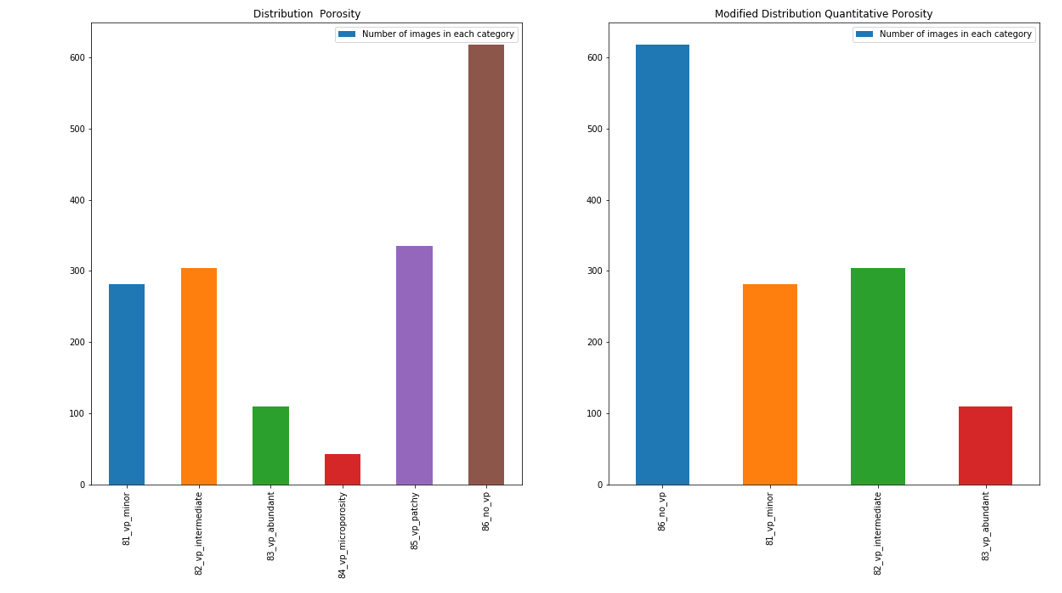
\includegraphics[width=1\linewidth]{figures/03-porosity_baby.PNG}
  \caption{Porosity Labels}
  \label{fig:porolab}
\end{subfigure}
\begin{subfigure}{.6\textwidth}
  \centering
  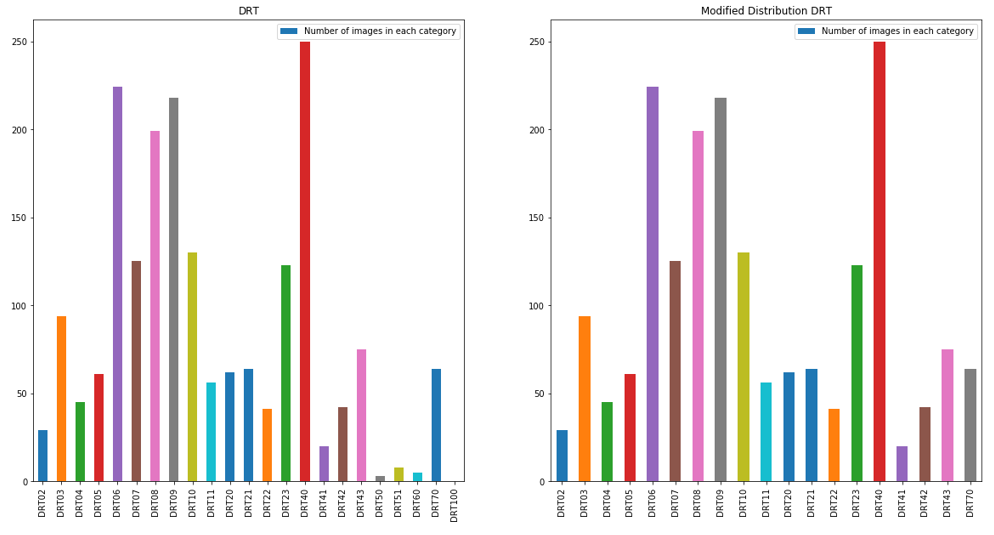
\includegraphics[width=1\linewidth]{figures/03-DRT.PNG}
  \caption{DRT Labels}
  \label{fig:drtlab}
\end{subfigure}%
\begin{subfigure}{.6\textwidth}
  \centering
  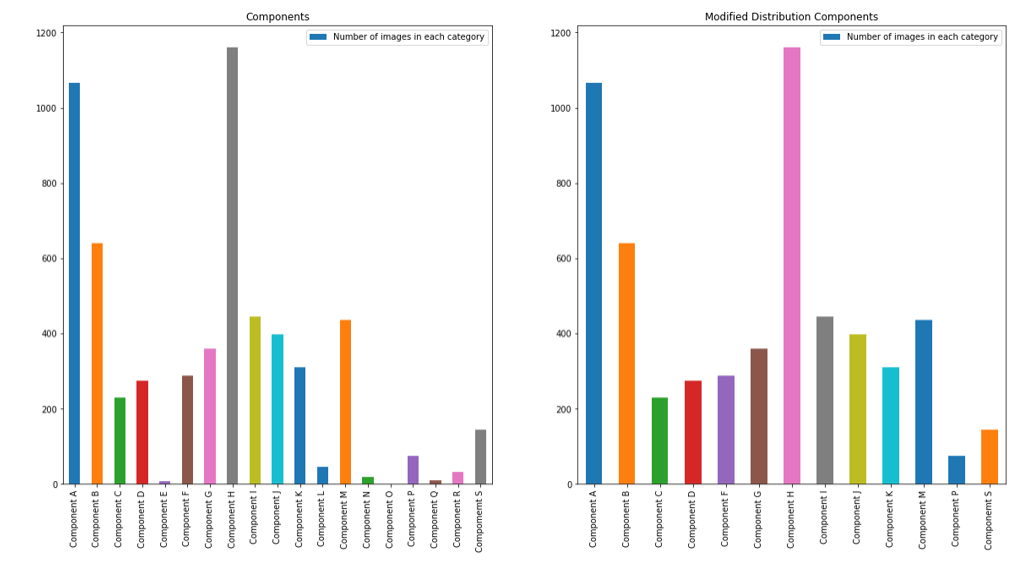
\includegraphics[width=1\linewidth]{figures/03-Components.PNG}
  \caption{Components Labels}
  \label{fig:compolab}
\end{subfigure}
\caption[Pre processing of labels]{Label distributions before and after pre-processing. Some labels are cut out,  the order can be re-arranged in order to produce more powerful visualization}
\label{fig:labelsdistrib}
\end{figure}

\subsection{Data Augmentation}
%% Editing note: \url{http://www.sepmstrata.org/microscopic_gallery_details.aspx?gid=224&pg=2&gcid=10} is where I took pictures from. 
The networks used for this thesis are trained on data set of around 10,000,000 images. Our data set has 1907 images, this difference makes it likely that we will not have enough sample for our network to learn properly. A way for us to get more training data is to use data augmentation.  There is a  large number of techniques that can be used. As mentioned in Section \ref{sec:dataug}, the most common are rotations, flips, resizing, rescaling, cropping and adding of noise. But some of them can not be used in our case. 

Cropping is a great way to create multiple images from one image. But there is a risk to crop only an irrelevant zone of the image. When classifying Components for example, in Figure~\ref{fig:crops}, we can see what could go wrong when cropping. Indeed, both images generated from the green and the yellow crops will have the same labels. The organism in the yellow crop is one of the components of the thin section, it will thus be one of the labels of the image. This means that both images will have this component as label, but it is not present in the second image. So we will teach our model the wrong information. A way of dealing with this would be to make big crops, so we keep most of the valuable information in each cropped image.  

\begin{figure}[h]
    \centering
        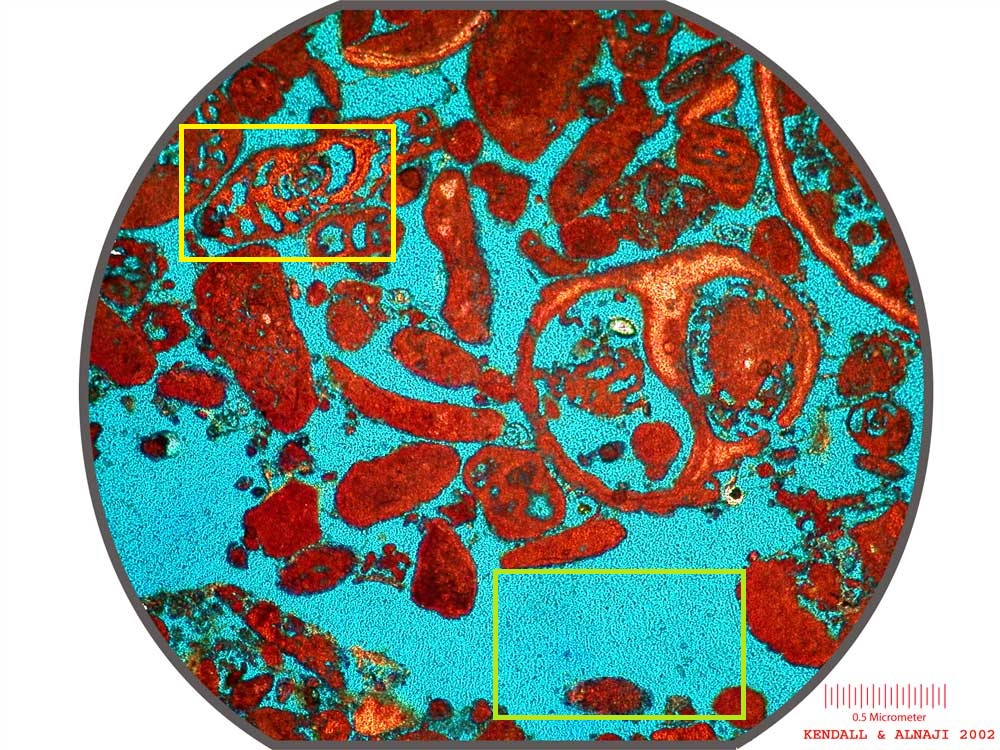
\includegraphics[width=0.5\textwidth]{figures/03-cropping_example_with2crops}
        \caption[Thin section with 2 random crops]{ Thin section with two random crops. The yellow and green crops have the same labels but contains very different information. This image has been adapted from \cite{section} which has a gallery of thin sections of carbonate rocks. }
        \label{fig:crops}
\end{figure}

When coring, a blue resin is injected into the core in order to keep fragments together. It also allows to see pores more clearly. It is thus important to maintain this blue color when doing data augmentation. That is why we can not change the colors in our images, techniques such as grayscale are discarded.


The augmentations used in this thesis are :
\begin{itemize}
    \item Color Jitter: In section \ref{sec:dataug}, we explained the way color jitter works. Now in Figures~\ref{fig:brightness} to ~\ref{fig:hue}, one can see how each parameters influence the image.
    We chose to keep all the parameters to 0.20. Except for hue that was kept to 0 since it is important to keep the colors unchanged. These values should remain small because we do not want to alter the image too much. If we do so, when we present it with new images, it will not be able to recognize them. 

\begin{figure}
\begin{subfigure}{.5\textwidth}
  \centering
  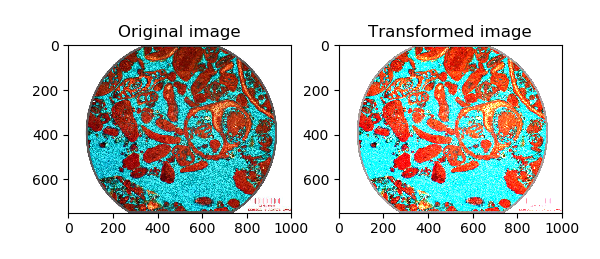
\includegraphics[width=1\linewidth]{figures/03-bightness08.PNG}
  \caption{Brightness= 0.2}
  \label{fig:brightness}
\end{subfigure}%
\begin{subfigure}{.5\textwidth}
  \centering
  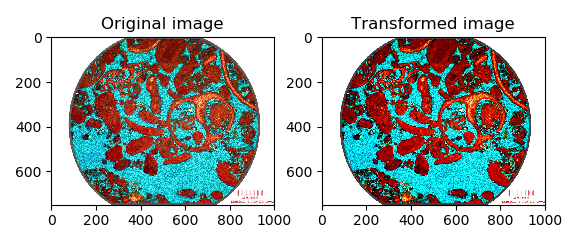
\includegraphics[width=1\linewidth]{figures/03-contrast1.PNG}
  \caption{Contrast = 0.2}
  \label{fig:contrast}
\end{subfigure}
\begin{subfigure}{.5\textwidth}
  \centering
  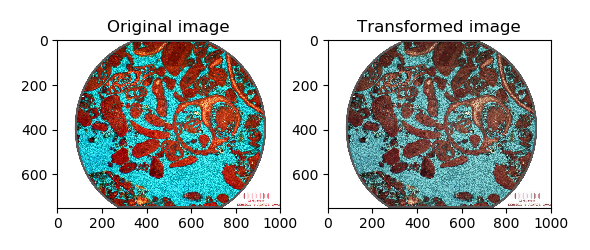
\includegraphics[width=1\linewidth]{figures/03-saturation0.PNG}
  \caption{Saturation = 0.2}
  \label{fig:saturation}
\end{subfigure}%
\begin{subfigure}{.5\textwidth}
  \centering
  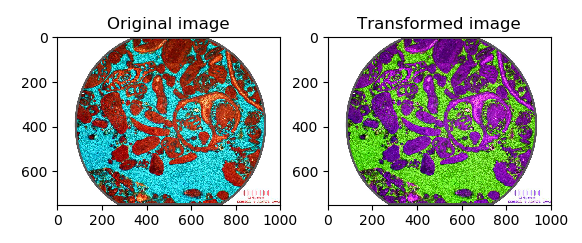
\includegraphics[width=1\linewidth]{figures/03-hue05.PNG}
  \caption{Hue = 0.5}
  \label{fig:hue}
\end{subfigure}
\caption[Color Jitter Augmentation]{Images before and after being augmented with ColorJitter. The parameter indicated under the image is the only one that is not set to 0. It shows the impact of different the parameters of ColorJitter. The images have been adapted from a thin section collected at \cite{section}}
\label{fig:colorjitter}
\end{figure}

    \item Rotation: This was the first data augmentation technique we used. The images in our data set are thin sections pictures of core. The core that is drilled out is a cylinder, so the pictures are round. In order to focus on the relevant pixels, all the pixels outside of the circle have been put to 0. This also allowed to be able to rotate the image as much as we want. The way we actually proceed is that we draw a number between 0 and 360. This number is the angle at which we rotate the picture. In Figure~\ref{fig:rotate}, we see how the rotation combined with a circle crop look.
\begin{figure}
\begin{subfigure}{.5\textwidth}
  \centering
  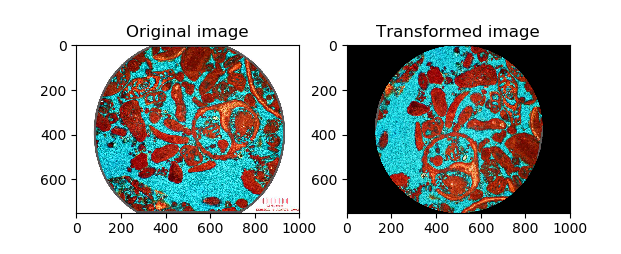
\includegraphics[width=1\linewidth]{figures/03-rotation_260}
  \caption{Circle crop and 260 degrees rotation}
  \label{fig:rotate}
\end{subfigure}%
\begin{subfigure}{.5\textwidth}
  \centering
  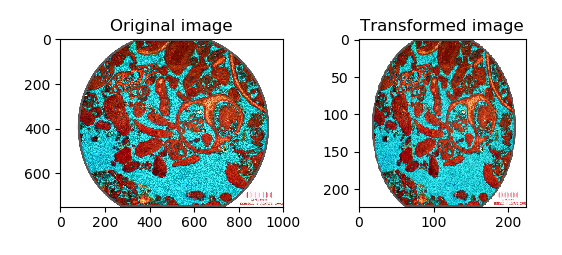
\includegraphics[width=1\linewidth]{figures/03-resize.PNG}
  \caption{Resizing to 224x224 pixels}
  \label{fig:resize}
\end{subfigure}
\begin{subfigure}{.5\textwidth}
  \centering
  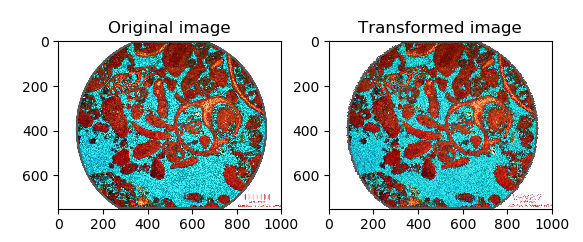
\includegraphics[width=1\linewidth]{figures/03-elastic_trans_08_03.PNG}
  \caption{Elastic Transform with (\(\alpha\)=3, \(\sigma\)=0.3)}
  \label{fig:elastics1}
\end{subfigure}%
\begin{subfigure}{.5\textwidth}
  \centering
  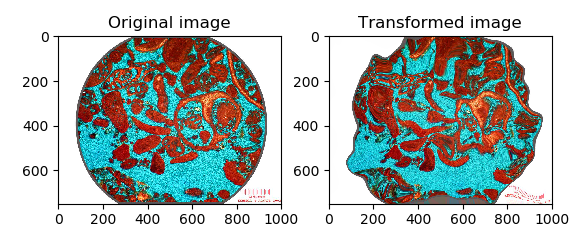
\includegraphics[width=1\linewidth]{figures/03-elastic_trans_3000_30.PNG}
  \caption{Elastic Transform with (\(\alpha\)=3000, \(\sigma\)=30)}
  \label{fig:elastics2}
\end{subfigure}
\begin{subfigure}{.5\textwidth}
  \centering
  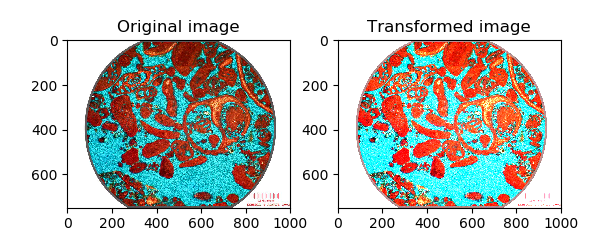
\includegraphics[width=1\linewidth]{figures/03-medianscale}
  \caption{Median Scale}
  \label{fig:median}
\end{subfigure}
\caption[Various data augmentation]{Images before and after being augmented with various Data Augmentations. We perform all of them on the original sized image to make it more visible. But in practice we perform the resizing first, to optimize our computation time. These images have been adapted from a thin section collected at \cite{section}}
\label{fig:transfos}
\end{figure}

    \item Resizing: The pictures were initially 5000x5000 pixels. We resized them to sizes usable by different models (224x224 for ResNet-18, 299x299 for Inception\_v3). This implies a loss in image quality but it drastically increases the speed of computation. See Figure~\ref{fig:resize}
    \item Elastic Transform : In Figure~\ref{fig:elastics1} and~\ref{fig:elastics2} , we have examples of two different sets of coefficients. The elastic transform on the first images looks more like adding some noise to the picture while the one on the right is extremely distorted. In our case, we can not use the second set of coefficients since we don't want to deform components so much that they are not identifiable any more. 

    \item Median Scale : This scales with the median and the mean of each channel (red, green and blue) of the numpy array. This gives a more clear view of the picture as shown in Figure~\ref{fig:median}  
 \end{itemize}

After Data Augmentation, we have a dataset of 19070 images. 


\section{Experiments}
\subsection{Inception\_v3}
We use the Inception\_v3 version of the GoogLeNet. It is the latest version implemented and available on PyTorch, this is why we chose this version. The network is 22 layers deep, 27 if we count the pooling layer. A detailed view of its architecture is shown in Figure \ref{fig:googarch}.
We repeat 2D convolutions paired with batch normalization with various kernel sizes. Before the final fully connected layer, we also have a pooling layer. The inception module is as described in section \ref{sec:gogl}. We display a part of it to show how the kernel size is changed.  
\subsection{ResNet}
%% Editing note : (research paperResNet or imagenet webpage
ResNet is the network that gives theoretically the best results \cite{resnetpaper}. There are different versions of this network with different depths: ResNet-18, ResNet50, ResNet101 etc... But we must keep in mind that we have a small data set compared to what is usually used for those networks. After data augmentation, we have around 19000 images. It is still far from ImageNet, so we should be careful about over-fitting. We can't use a too deep network on a small amount of data. That is why we chose to only use ResNet-18. The architecture is presented in Figure~\ref{fig:resarchi}

After a first convolution layer, we use a basic block as shown in Figure~\ref{fig:resarchi} that we repeat until the last layer. In this last layer, out\_features is the number of classes the network should output. 
\subsection{AlexNet}
AxelNet is a smaller network, only eight layers deep, so the lack of training data is not so critical in this case. It is divided in two parts: five convolutional layers to do the feature extraction and three linear layers to do the classification.  The details of the architecture are shown in Figure~\ref{fig:resarchi}
\begin{figure}
\begin{subfigure}{.5\textwidth}
  \centering
  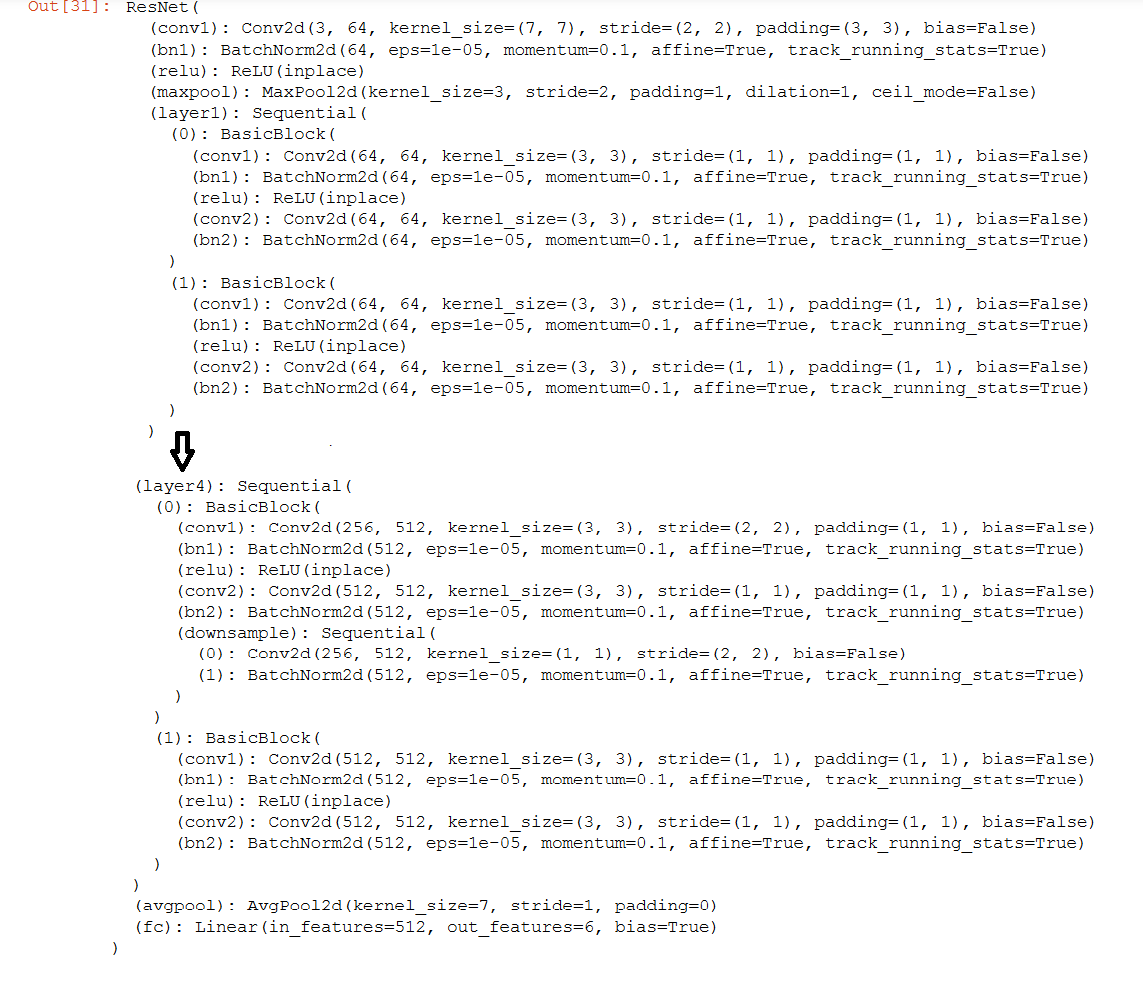
\includegraphics[width=6cm, height=3cm]{figures/03-Resnet_architecture.png}
  \caption{ResNet-18}
  \label{fig:resarchi}
\end{subfigure}%
\begin{subfigure}{.5\textwidth}
  \centering
  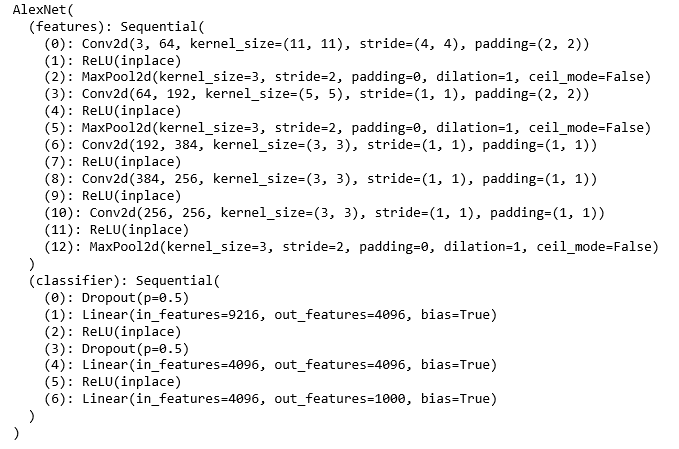
\includegraphics[width=6cm, height=3cm]{figures/03-alexnet_architecture}
  \caption{AlexNet}
  \label{fig:alexarchi}
\end{subfigure}
\begin{subfigure}{.5\textwidth}
  \centering
  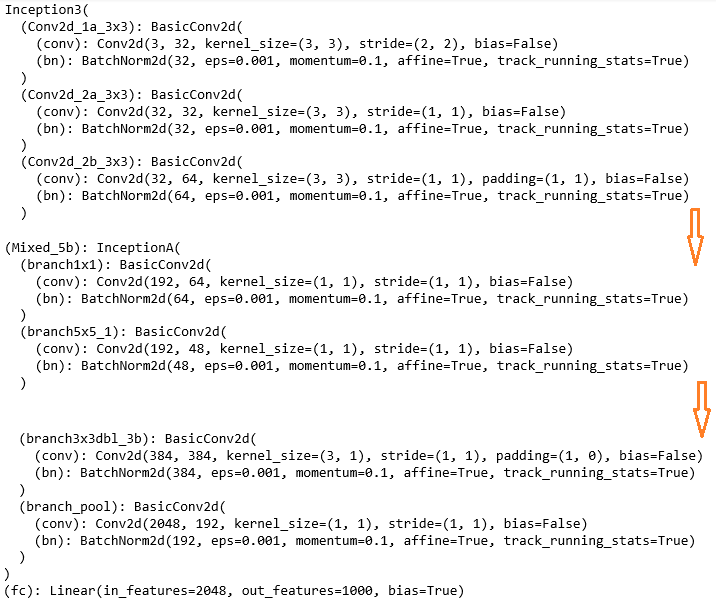
\includegraphics[width=6cm, height=3cm]{figures/03-inception_architecture}
  \caption{Inception\_v3}
  \label{fig:googarch}
\end{subfigure}
\caption[Networks architectures]{The architectures of the three networks. AlexNet is a simple eight layers network divided in two parts: feature extraction and classification. ResNet-18 is a deep network with a basic block repeated several times and a single linear layer in the end. Inception\_v3 is a 22 deep \gls{cnn} with repeated Inception blocks.}
\end{figure}

\subsection{Hyper parameters}
Hyper parameters are the parameters that are chosen before training, and that will remain the same during the whole training. One of the questions in this thesis is to study the influence of some hyper parameters on the  convergence of the algorithm. To do so, we will make some of them may vary from one experiment to an other. 


\subsubsection{Weights initialization} \label{sec:init}
As mention in Section \ref{sec:translearn}, there are two ways of using the networks to perform a classification task. Either you train all the layers in the network and randomly initialize the weights. Or we use the weights that have achieved good results on known data set and retrain only a smaller part of the network to make it specific to the task.
Choosing between those two tasks depends on the size of the network and the size of the data set. If the network is too deep, training all the layers might lead to over-fitting. But if the data set is very big, then we need to train the whole model to make it recognize forms in our data set. 
We will conduct two trainings in parallel for each class. One with random initialization and one with pretrained weights. 
When conducting those experiments, we use the Adam optimizer since we want to converge quickly to a minimum to compare the two approaches. 

After this first experiment, we will determine which networks performs best. We will also test the hypothesis that every class performs similarly with one specific network. So for example, if ResNet-18 performs better with pretrained weights on the Dunham class, it will do so also on the porosity class. This way we do not need to optimize our network on every one of the 4 classes. 

\subsubsection{Batch size}
The batch sized is fixed to 700 so that two experiments can be run in parallel on the same GPU for ResNet-18 and AlexNet. For Inception\_v3, the batch size is set to 50 to be able to run two experiments in parallel. In case we need to run more than two experiments in parallel, we reduce the batch size accordingly.

\subsubsection{Train/Test split}
In order to monitor the performances of our algorithm, we split the data set in three parts. 80\% of the data is used for training, 10\% is used for validation and 10\% for test. The 10\% used for test are not used at all during the training. It is only used when to do predictions on to see how our network is performing on "new" data. 

\subsubsection{Optimizers}
For Adamax, there is a set of default values for the hyper-parameters: \(\eta = 0.002\), \(\beta_1 = 0.9\) \(\beta_2 = 0.999\), \(\epsilon = 1e-8\) that we will keep across all experiments. We kept those from the default configuration of the optimizer. 
For the \gls{sgd}, we choose an initial value of learning rate in [0.1, 0.01, 0.001] and implemented a learning rate decay every 30 iterations, and a momentum of 0.9. 

Adamax is used to get a good convergence quickly, this is why we use Adamax in the first experiment on the weight initialization. This first experiment is going to give us insight on which network performs best on the different labels. Then in a second experiment, we will try to optimize further the best performing model. To reach the best possible results We will use the \gls{sgd}+momentum optimizer. We can then check the influence of the optimizer on our results. 

\subsubsection{Regularization}
As we mentioned before, the small amount of data we have make over-fitting likely. In order to avoid this problem, we add a layer of dropout with probability 0.5 in AlexNet. ResNet-18 and Inception\_v3 already performs batch normalization between every convolutional. That is an efficient way of doing regularization. This is why we did not add any dropout layer.  
\chapter{Results}\label{chp:results}

In this chapter, we present the results of different networks. Sections from \ref{sec:res} to \ref{sec:gogl} present the results for each network. Every section is divided in two subsection: one in which we discuss the results of different initialization and one in which the results for different classes are presented. In Section \ref{sec:opt}, we present the results for a different optimizer and three learning rates. 
\section{ResNet-18}\label{sec:res}
\subsection{Initialization}
For every class, we tested our network with either random initialization or with using pretrained weights. In Table \ref{tab:resinit}, we can see the best accuracy on the validation set and the number of epochs for training for each class.  

\begin{table}
\caption[Results according to initialization of ResNet-18]{\label{tab:resinit} The results of training ResNet-18 using random initialization or pretrained weights with Adamax as optimizer. The score is the validation accuracy for Dunham, Porosity and \gls{drt}. It is the F1-score for the Components class.}
\centering
\begin{tabular}[b]{| l | l | l | l | l |}
\hline
    Initialization & Class & Validation score & Epochs\ \\ \hline
    \multirow{4}{*}{Pretrained Weights} & Dunham &  60,7\%  & 50 \\ 
    & Porosity & 73,8\%  &  60 \\
    &DRT & 52,1\% &  50 \\
    &Components & 69,1\% &  50 \\ \hline
     \multirow{4}{*}{Random} & Dunham &  44,8\%  & 50 \\
    & Porosity & 63,4\% &  50 \\
    &DRT & 27,6\% & 50 \\
    &Components & 34,1\% &  50 \\ \hline
    
\end{tabular} 
\end{table}
In Figure \ref{fig:plotres}, we plotted the accuracy, F1 score, and average training and validation loss for each class. 


\begin{figure}
\makebox[\linewidth][c]{%
\begin{subfigure}[b]{.6\textwidth}
\centering
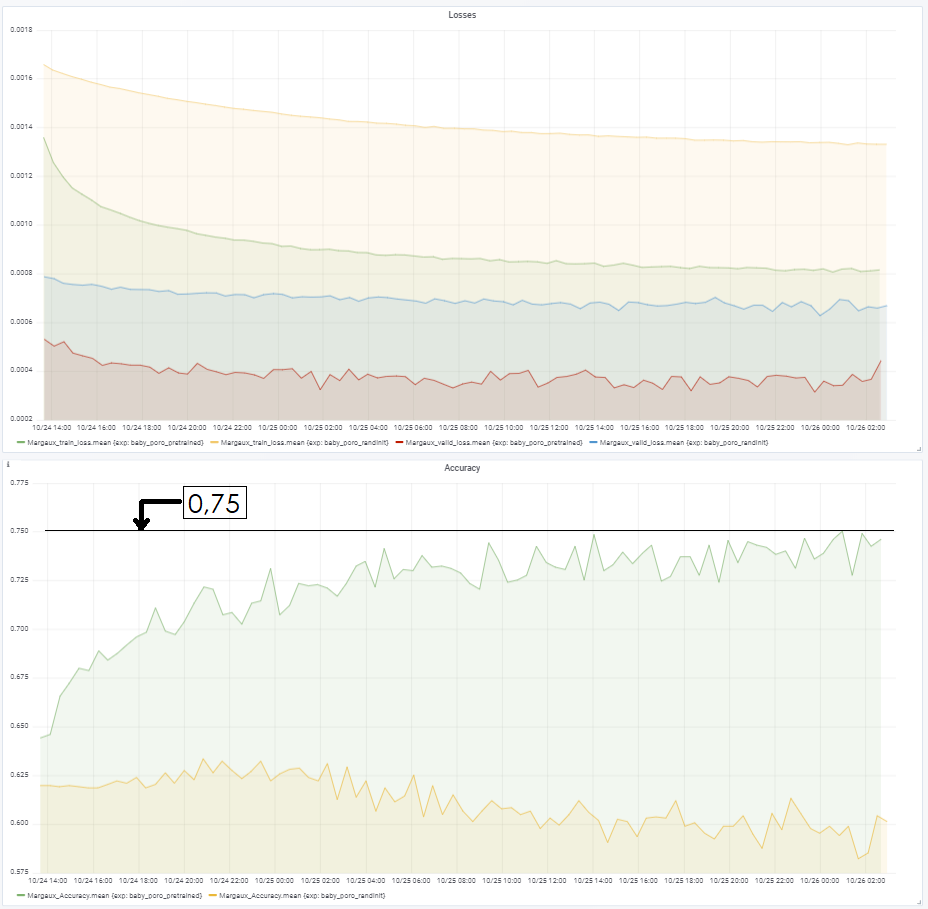
\includegraphics[width=.95\textwidth]{figures/04-Init_poro_acc.PNG}
\caption{ResNet 18 trained on the Porosity class.}
\label{fig:resinitporo}
\end{subfigure}%
\begin{subfigure}[b]{.6\textwidth}
\centering
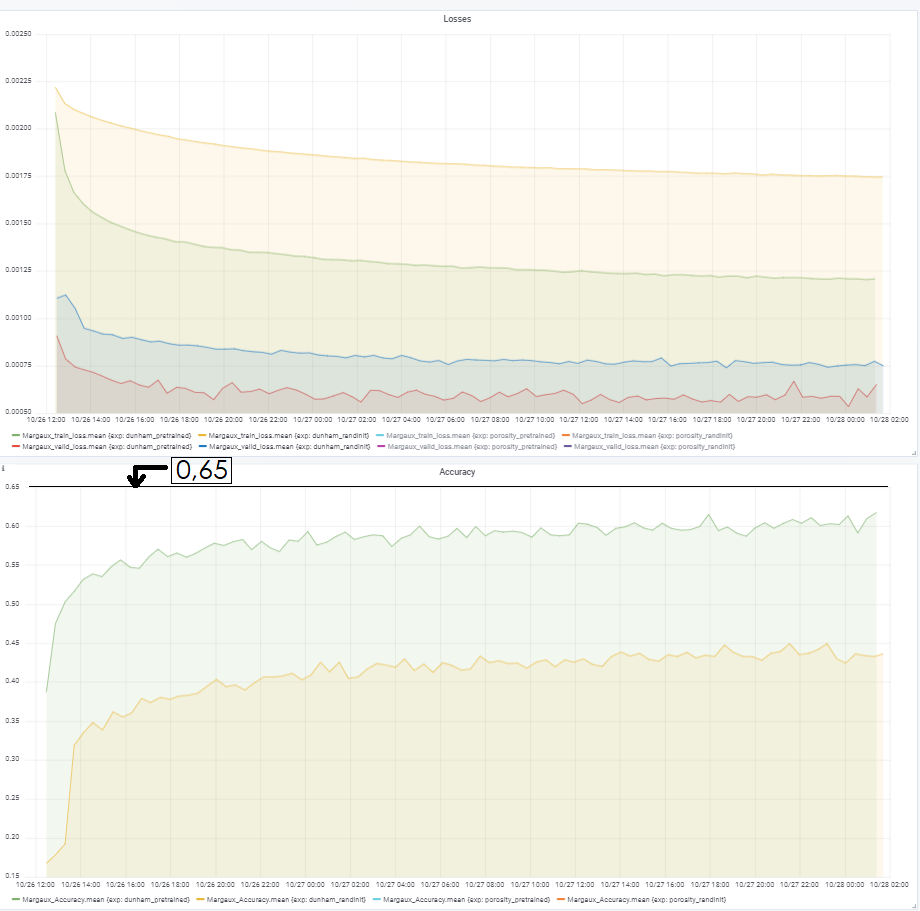
\includegraphics[width=.95\textwidth]{figures/04-Init_dunham_acc.PNG}
\caption{ResNet-18 trained on the Dunham class.}
\label{fig:resinit_dunham}
\end{subfigure}%
}\\
\makebox[\linewidth][c]{%
\begin{subfigure}[b]{.6\textwidth}
\centering
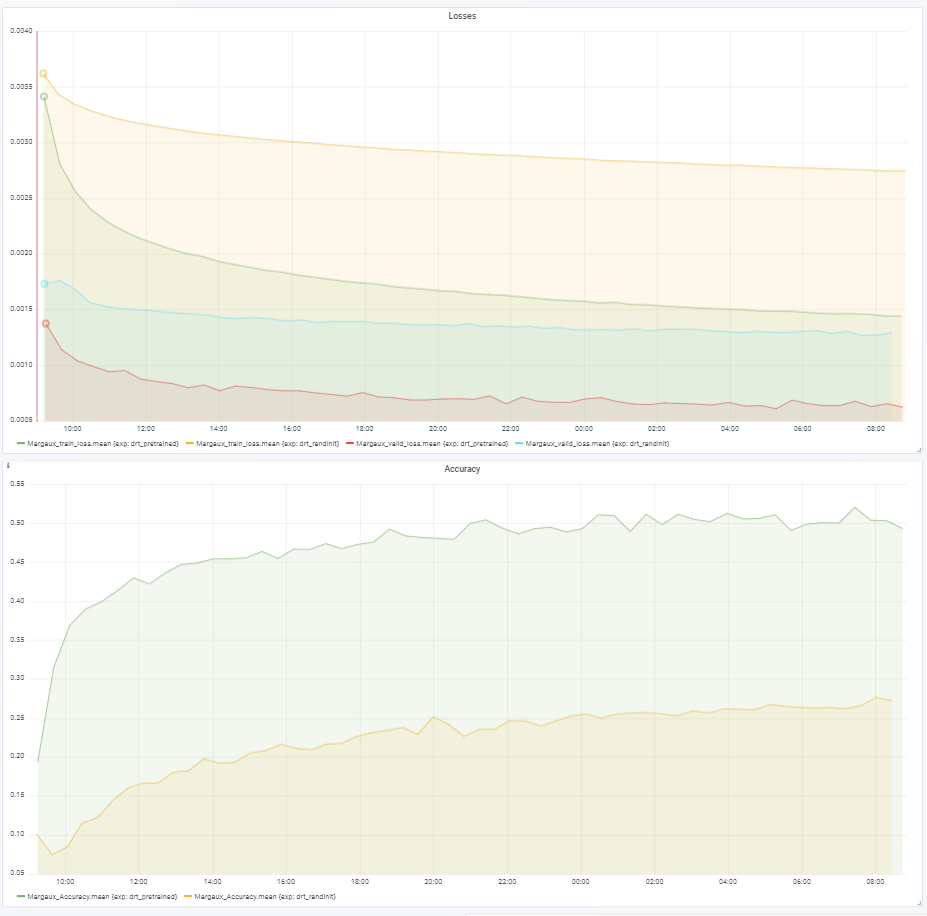
\includegraphics[width=.95\textwidth]{figures/04-Init_drt_acc.PNG}
\caption{ResNet-18 trained on the DRT class.}
\label{fig:resinit_drt}
\end{subfigure}%
\begin{subfigure}[b]{.6\textwidth}
\centering
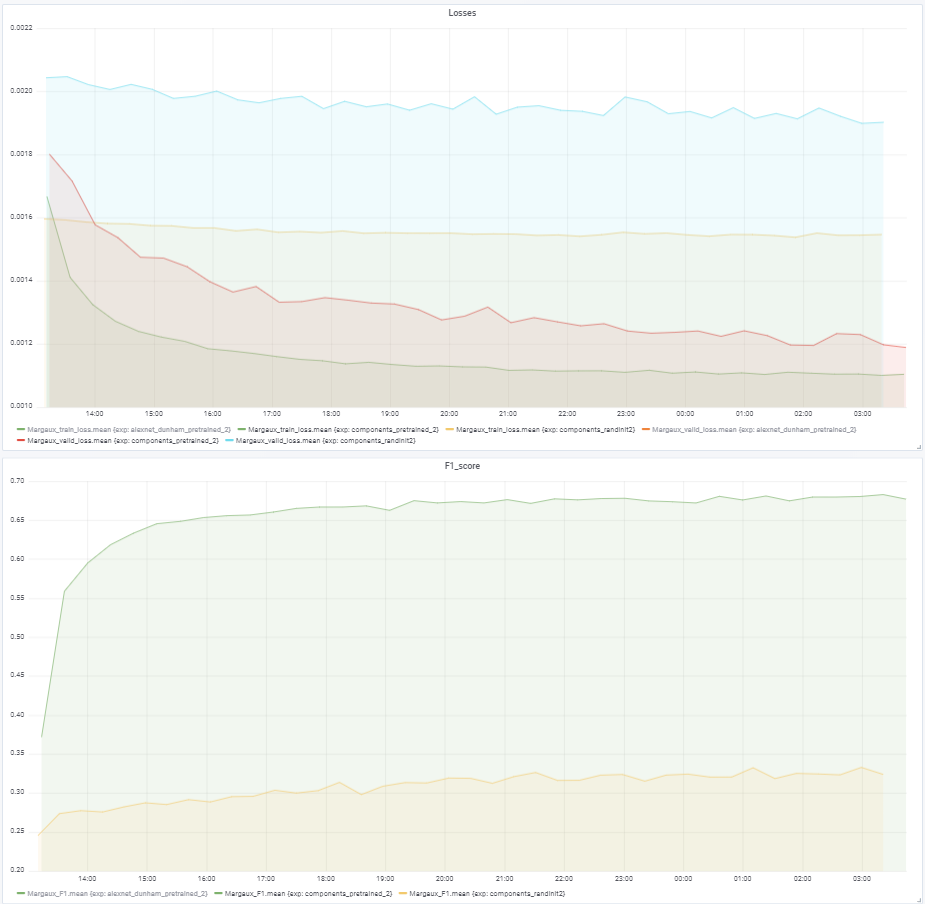
\includegraphics[width=.95\textwidth]{figures/04-Init_components_acc.PNG}
\caption{ResNet-18 trained on the Components class.}
\label{fig:resinit_comp}
\end{subfigure}%
}
\caption[Training and validation plots for ResNet-18]{The lines in green and red are for pretrained weights and yellow and blue for random initialization. The bottom plot is the validation accuracy for plots (a), (b) and (c) and the F1-score for plot (d). The top plot is training  and validation loss. At the top of the top plots, we show the value toward which the score converges.}
\label{fig:plotres}
\end{figure}

\subsection{Classification}
In Table \ref{tab:resbest}, we summarize the best validation and test accuracy or F-1 score for every class. Then we present the confusion matrix for the best performing model and the test data set for the single label classification in Figure \ref{fig:rescm}. For the Components class, we show the statistics for every class in Figure \ref{fig:perf_res}. 

\begin{table}
\caption[Scores of best performing ResNet-18]{\label{tab:resbest} The results of the best version of the ResNet-18 on the classification task. The validation and test accuracy are used as score on the single label classification while F1-scores are used for multi-label classification.}
\centering
\begin{tabular}[b]{| l | l | l | l | l |}
\hline
    Initialization & Class & Validation score & Test score \ \\ \hline
    Pretrained Weights & Dunham &  60,7\%  & 37,3\% \\ \hline
    Pretrained Weights & Porosity & 73,8\%  &  58,5\% \\ \hline
    Pretrained Weights &DRT & 52,1\% &  22,1\% \\ \hline
    Pretrained Weights &Components & 69,1\% &  44,7\% \\ \hline
\end{tabular} 
\end{table}

\begin{figure}
\makebox[\linewidth][c]{%
\begin{subfigure}[b]{.6\textwidth}
\centering
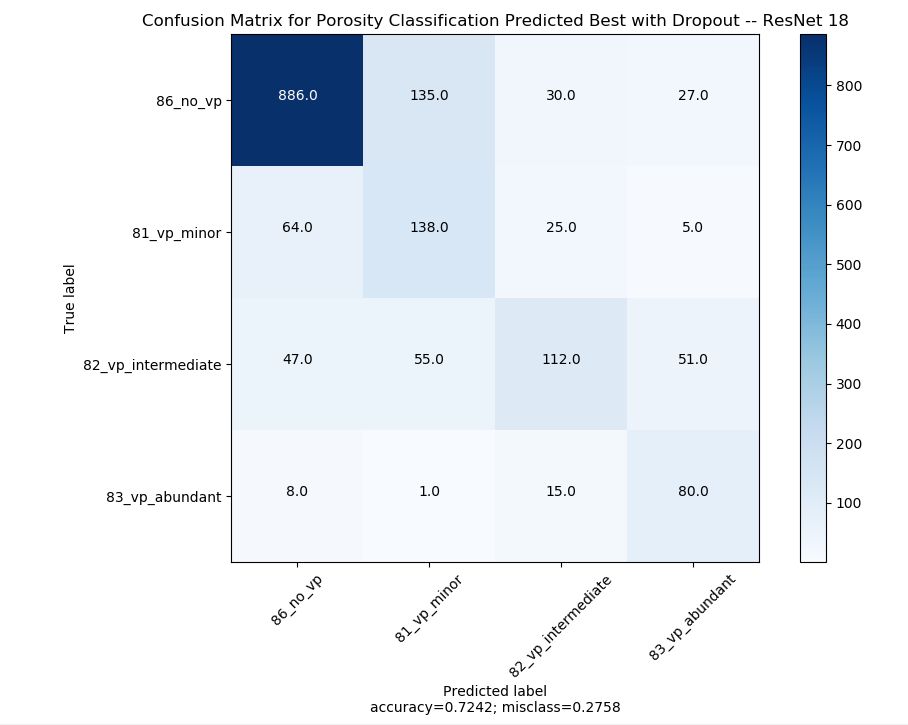
\includegraphics[width=.95\textwidth]{figures/04-baby_best.PNG}
\caption{Best for the Porosity class.}
\label{fig:rescm_poro}
\end{subfigure}%
\begin{subfigure}[b]{.6\textwidth}
\centering
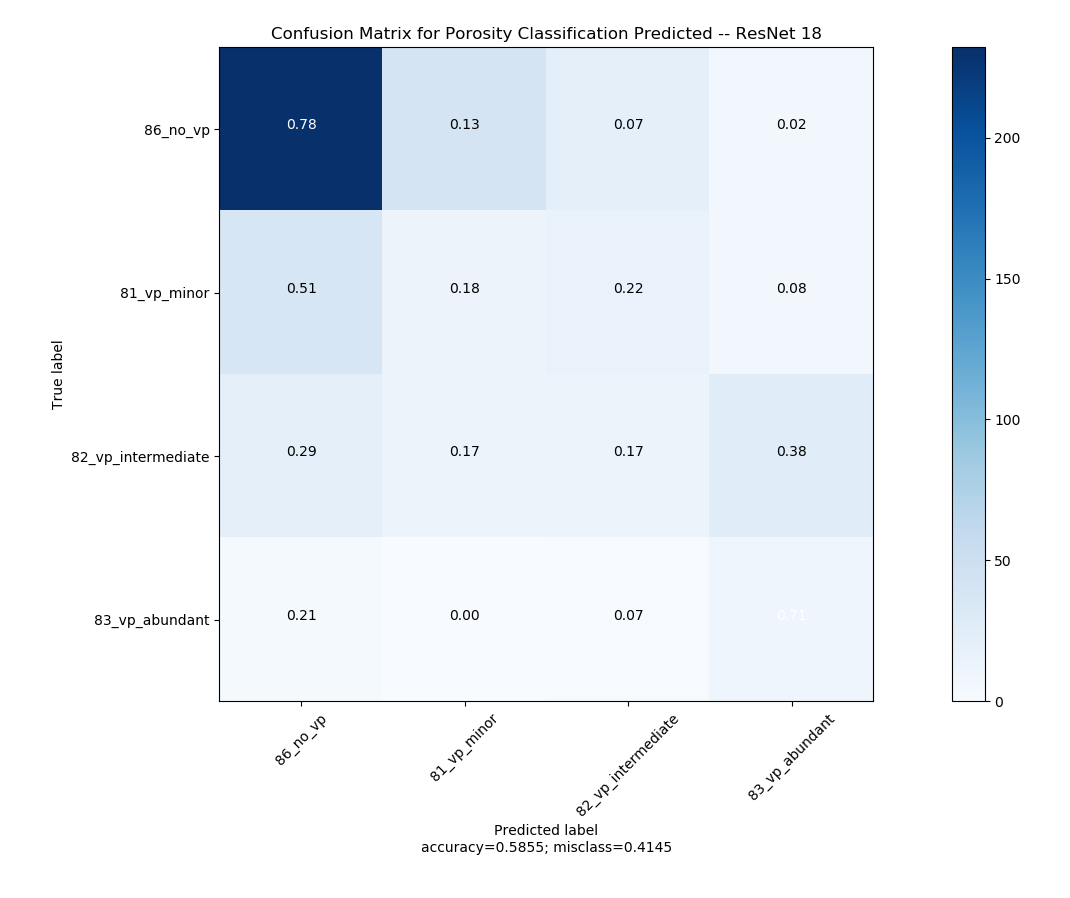
\includegraphics[width=.95\textwidth]{figures/04-baby_pred.PNG}
\caption{Predicted for the Porosity class.}
\label{fig:rescm_poro_pred}
\end{subfigure}%
}\\
\makebox[\linewidth][c]{%
\begin{subfigure}[b]{.6\textwidth}
\centering
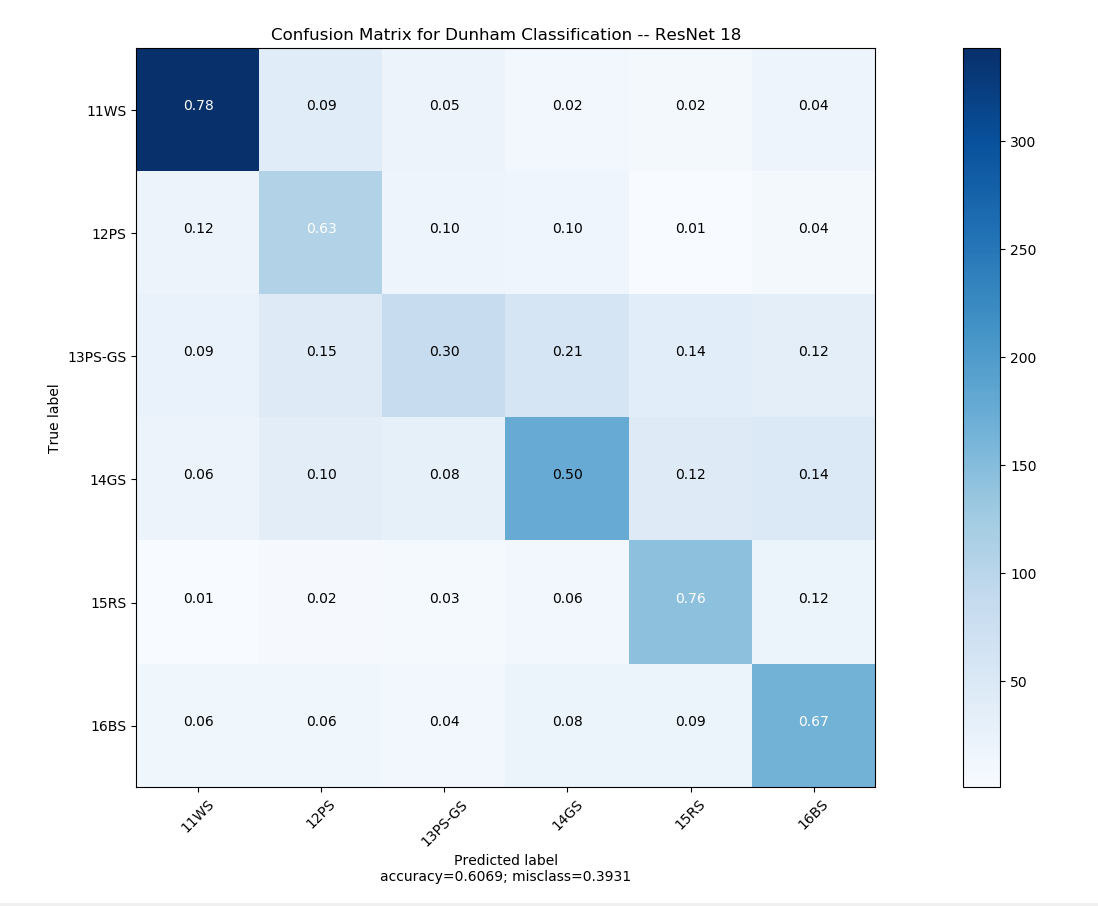
\includegraphics[width=.95\textwidth]{figures/04-dunham_best.PNG}
\caption{Best for the Dunham class.}
\label{fig:rescm_dunham}
\end{subfigure}%
\begin{subfigure}[b]{.6\textwidth}
\centering
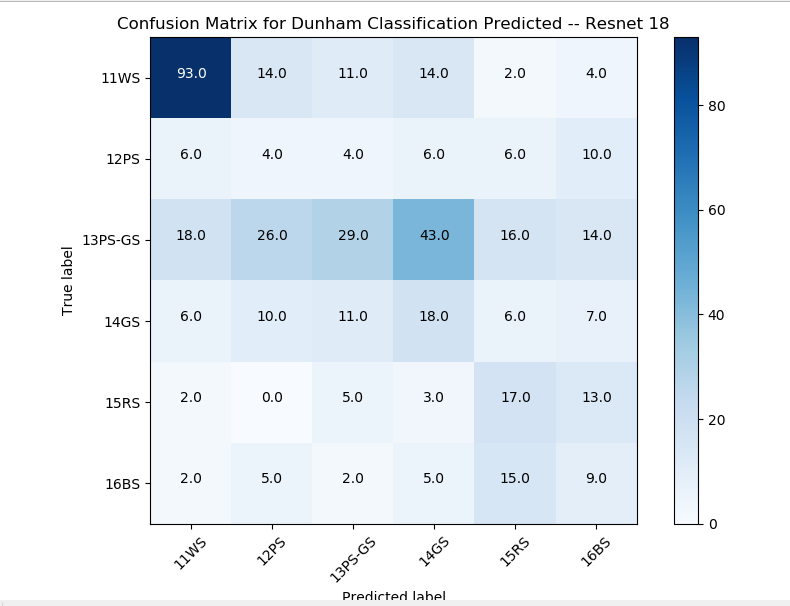
\includegraphics[width=.95\textwidth]{figures/04-dunham_pred.PNG}
\caption{Predicted for the Dunham class.}
\label{fig:rescm_dunham_pred}
\end{subfigure}%
}
\makebox[\linewidth][c]{%
\begin{subfigure}[b]{.6\textwidth}
\centering
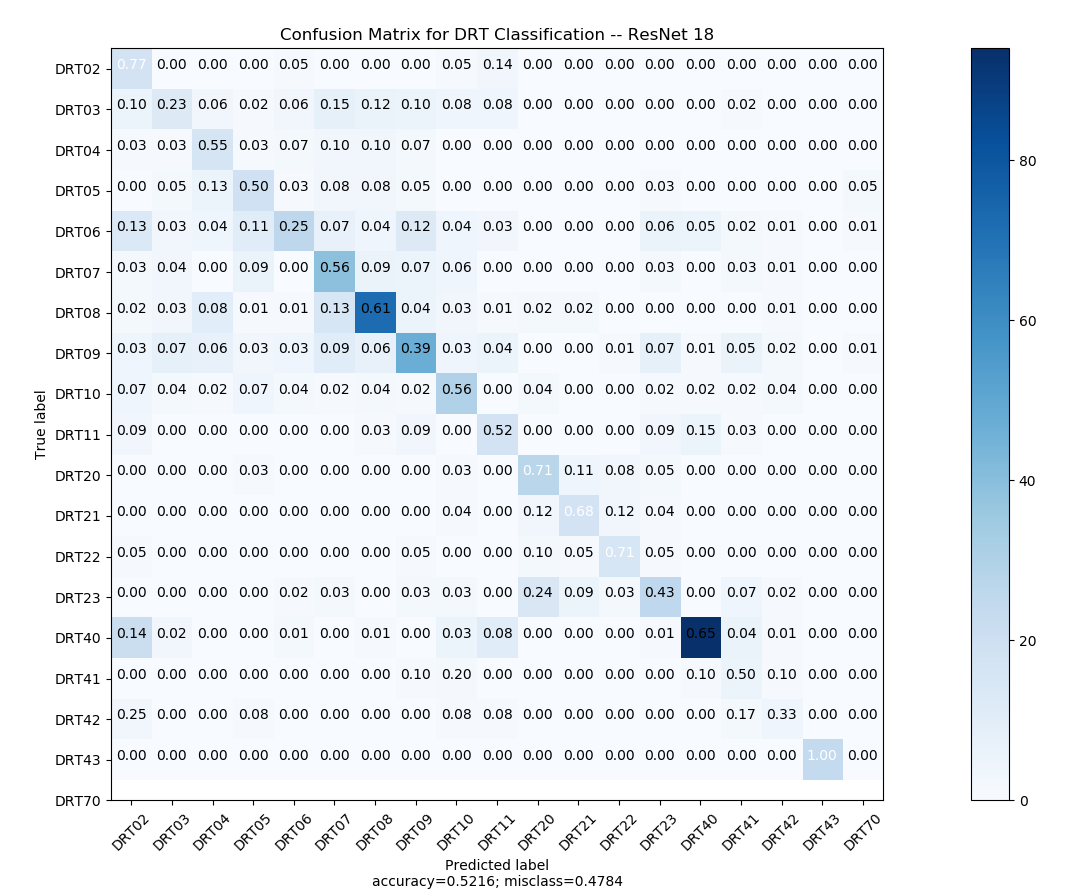
\includegraphics[width=.95\textwidth]{figures/04-drt_best.PNG}
\caption{Best for the DRT class.}
\label{fig:rescm_drt}
\end{subfigure}%
\begin{subfigure}[b]{.6\textwidth}
\centering
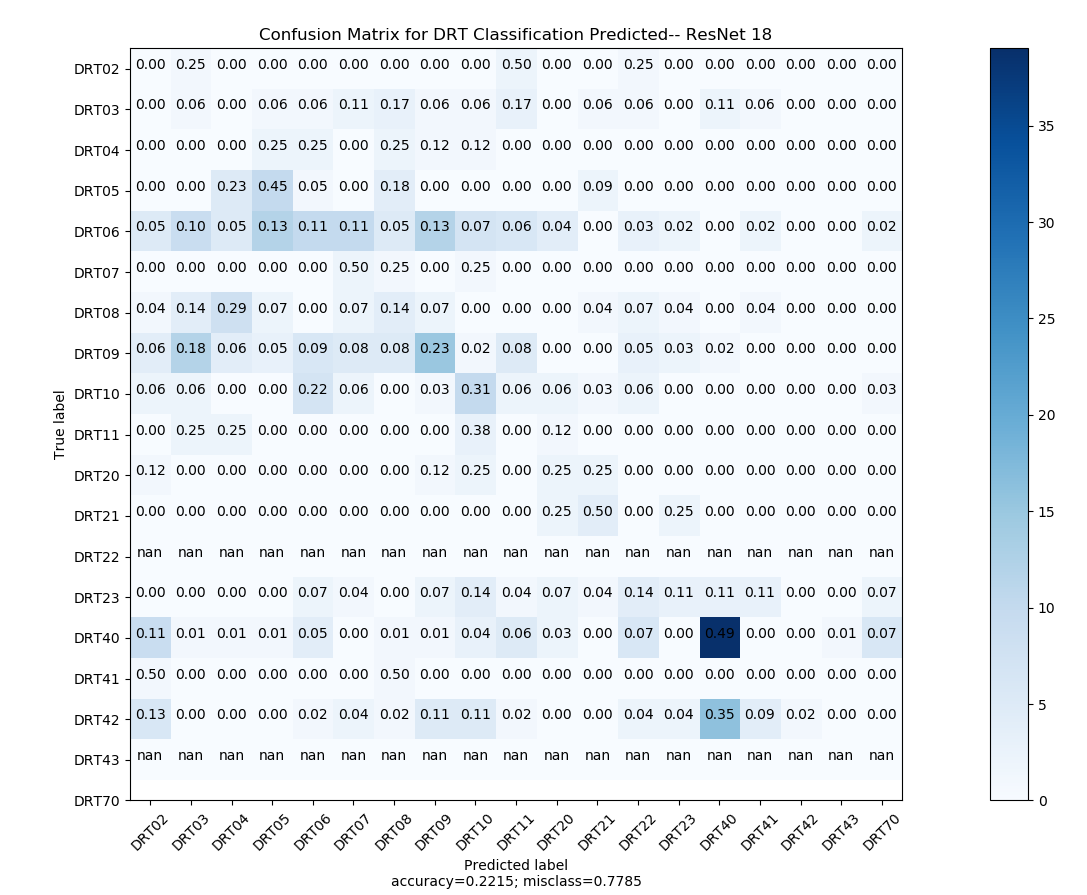
\includegraphics[width=.95\textwidth]{figures/04-drt_pred.PNG}
\caption{Predicted for the DRT class.}
\label{fig:rescm_drt_pred}
\end{subfigure}%
}
\caption[Confusion matrices of classes trained on ResNet-18]{On the left is the confusion matrix of the best performing ResNet-18 and on the right is the confusion matrix on the test set.}
\label{fig:rescm}
\end{figure}

\begin{figure}
\makebox[\linewidth][c]{%
\begin{subfigure}[b]{.6\textwidth}
\centering
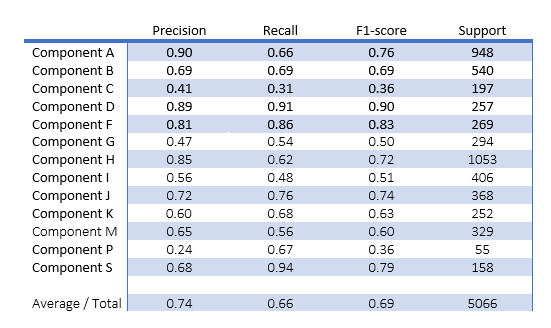
\includegraphics[width=.95\textwidth]{figures/04-compo_best.PNG}
\caption{Best for the Components class.}
\label{fig:rescm_comp}
\end{subfigure}%
\begin{subfigure}[b]{.6\textwidth}
\centering
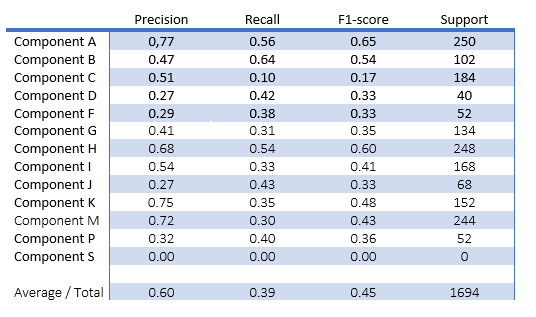
\includegraphics[width=.95\textwidth]{figures/04-compo_pred.PNG}
\caption{Predicted for the Components class.}
\label{fig:rescm_comp_pred}
\end{subfigure}%
}
\caption [Performance summary of the Components class trained on ResNet-18]{These figure are the summaries of the performance for the multi-label classification. It shows precision, recall, F1-score and also the number of samples for each class.}
\label{fig:perf_res}
\end{figure}


%%%%%%%%%%%%%%%%%%%%%%%%%%%%%%%%%%%%%%%%%%%%%%%%%%%   ALEX   %%%%%%%%%%%%%%%%%%%%%%%%%%%%%%%%%%%%%%%%%%%%%%%%%%%%%

\section{AlexNet}\label{sec:aleX}
\subsection{Initialization}
For every class, we tested our network with either random initialization or with using pretrained weights. In Table \ref{tab:alexinit}, we can see the best accuracy on validation and test set, the number of epochs for training for each class.  
In Figure \ref{fig:plotsalex}, we plotted the accuracy, F1 score, and average training and validation loss for each class. 
\begin{table}
\caption[Results according to initialization of AlexNet]{\label{tab:alexinit} The results of training AlexNet using random initialization or pretrained weights with Adamax as optimizer}
\centering
\begin{tabular}[b]{| l | l | l | l | l |}
\hline
    Initialization & Class & Validation accuracy  & Epochs\\ \hline
    \multirow{4}{*}{Pretrained Weights} & Dunham &  81,7\%  & 50 \\ %%cf Confusion Matrix 
    & Porosity & 88,5\% &  50 \\
    &\gls{drt} & 74,5\% &  50 \\
    &Components & 85,1\% &  50 \\ \hline
     \multirow{4}{*}{Random} & Dunham &  62,1\% & 50 \\
    & Porosity & 64,8\% &  50 \\
    &\gls{drt} & 60,7\% &  50 \\
    &Components & 72,3\% & 50 \\ \hline
\end{tabular} 
\end{table}

\begin{figure}
\makebox[\linewidth][c]{%
\begin{subfigure}[b]{.6\textwidth}
\centering
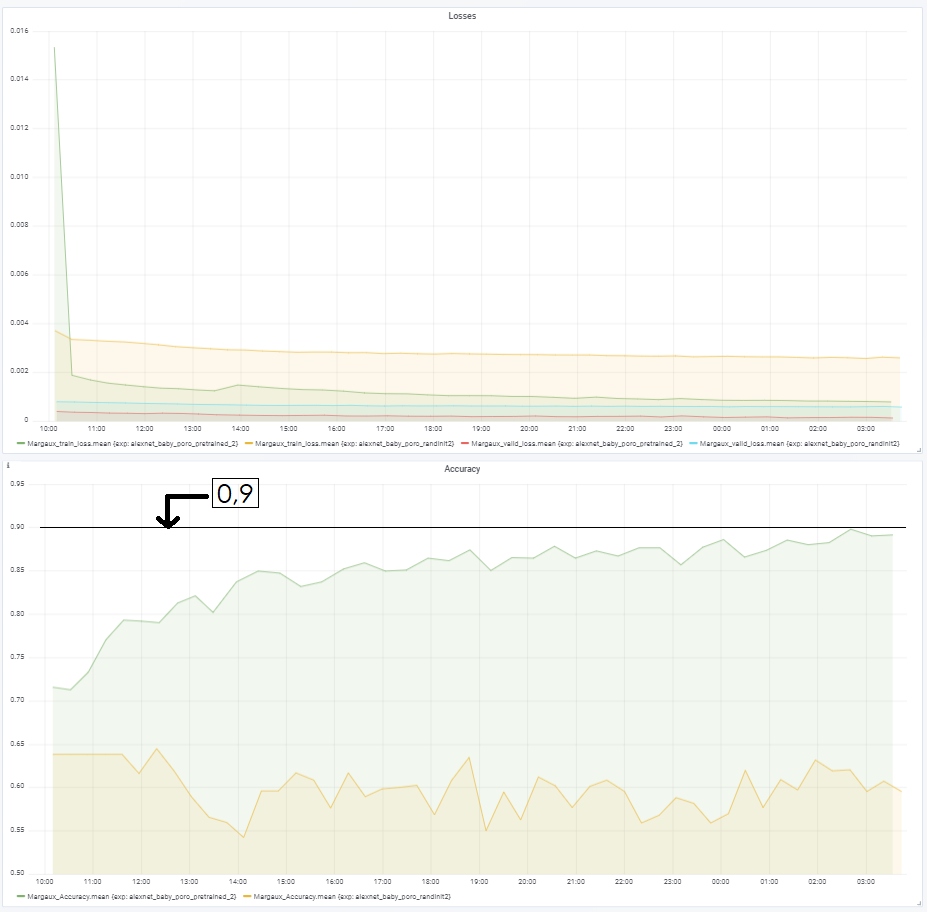
\includegraphics[width=.95\textwidth]{figures/04-Init_al_poro_acc.PNG}

\caption{AlexNet trained on the Porosity class.}
\label{fig:alexinit_poro}
\end{subfigure}%
\begin{subfigure}[b]{.6\textwidth}
\centering
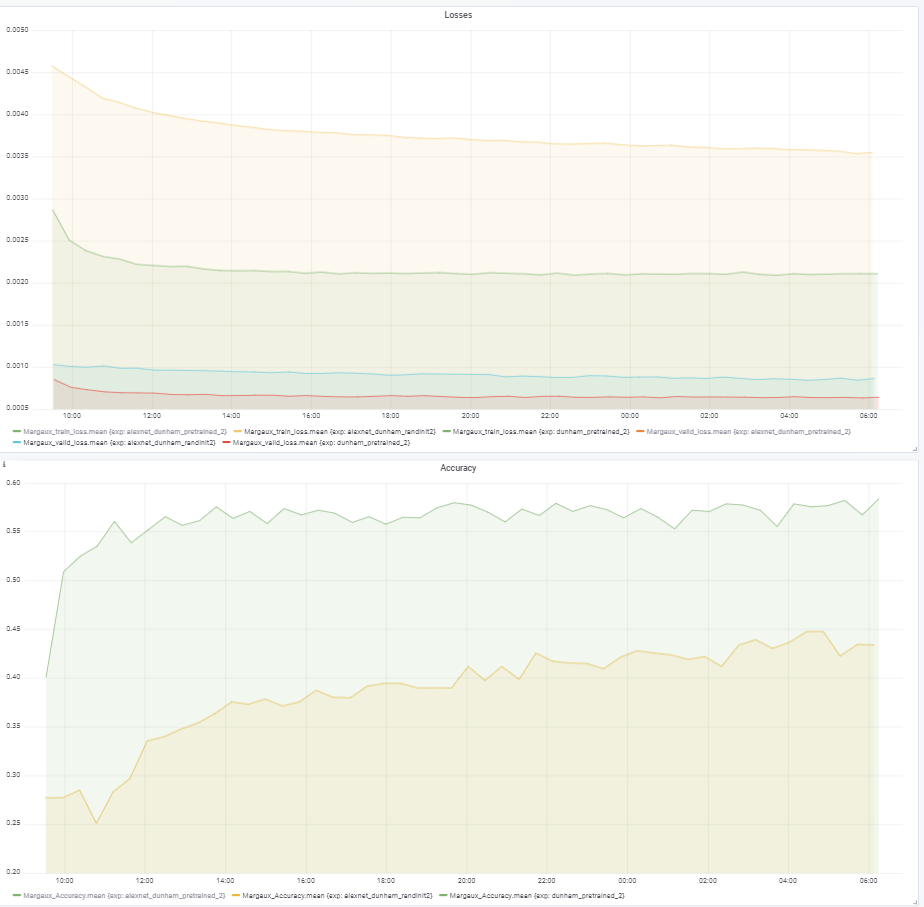
\includegraphics[width=.95\textwidth]{figures/04-Init_al_dunham_acc.PNG}
\caption{AlexNet trained on the Dunham class.}
\label{fig:alexinit_dunham}
\end{subfigure}%
}\\
\makebox[\linewidth][c]{%
\begin{subfigure}[b]{.6\textwidth}
\centering
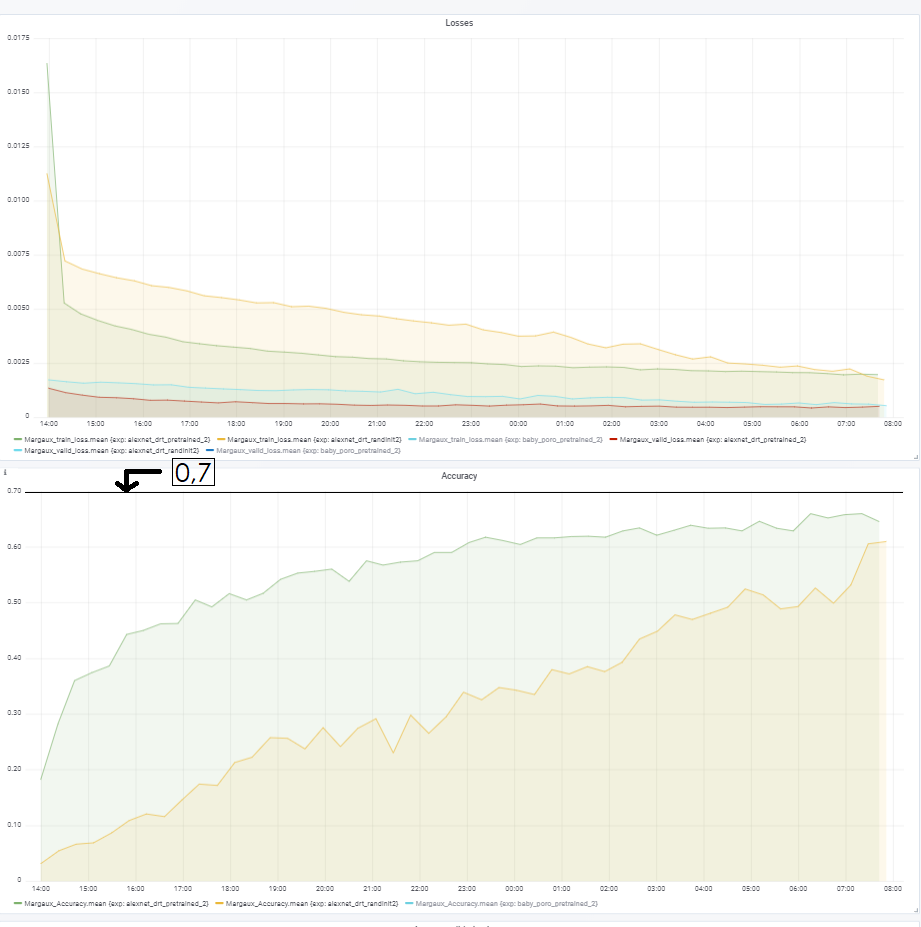
\includegraphics[width=.95\textwidth]{figures/04-Init_al_drt_acc.PNG}
\caption{AlexNet trained on the \gls{drt} class.}
\label{fig:alexinit_drt}
\end{subfigure}%
\begin{subfigure}[b]{.6\textwidth}
\centering
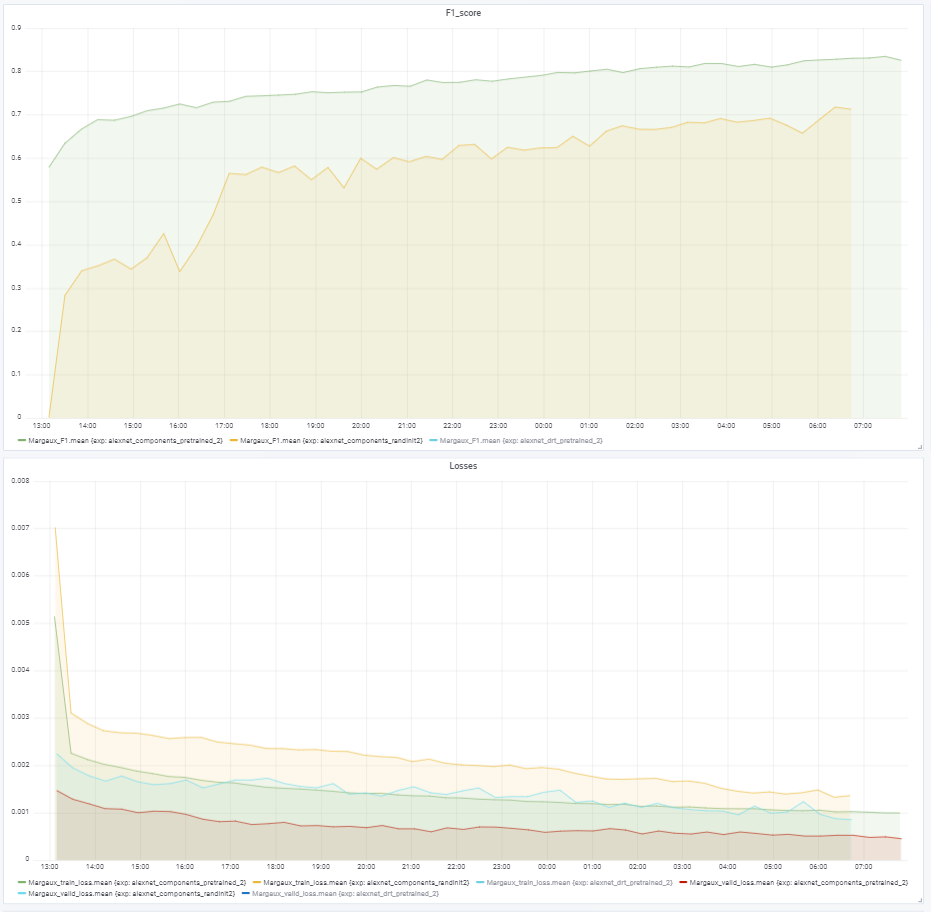
\includegraphics[width=.95\textwidth]{figures/04-al_components_acc.PNG}
\caption{AlexNet trained on the Components class.}
\label{fig:alexinit_comp}
\end{subfigure}%
}
\caption[Training and validation plots for AlexNet]{The lines in green and red are for pretrained weights and yellow and blue for random initialization. The bottom plot is the validation accuracy for plots (a), (b) and (c) and the F1-score for plot (d). The top plot is training  and validation loss. At the top of the top plots, we show the value toward which the score converges.}
\label{fig:plotsalex}
\end{figure}


\subsection{Classification}
In Table \ref{tab:alexbest}, we summarize the best validation and test accuracy or F-1 score for every class. Then we present the confusion matrix for the best performing model and the test data set for the single label classification in Figure \ref{fig:alcm}. For the Components class, we show the statistics for every class in Figure \ref{fig:perf_al}. 

\begin{table}
\caption[Scores of best performing AlexNet]{\label{tab:alexbest} The results of the best version of the AlexNet on the classification task. The validation and test accuracy are used as score on the single label classification while F1-scores are used for multi-label classification.}
\centering
\begin{tabular}[b]{| l | l | l | l | l |}
\hline
    Initialization & Class & Validation score & Test score  \\ \hline
    Pretrained Weights & Dunham &  81,7\%  & 36,8\% \\ \hline
    Pretrained Weights & Porosity & 88,5\%  &  69,5\% \\ \hline
    Pretrained Weights &\gls{drt} & 74,5\% &  23,4\% \\ \hline
    Pretrained Weights &Components & 85,1\% &  50,2\% \\ \hline
\end{tabular} 
\end{table}

\begin{figure}
\makebox[\linewidth][c]{%
\begin{subfigure}[b]{.6\textwidth}
\centering
\includegraphics[width=.95\textwidth]{figures/04-al_baby_best.PNG}
\caption{Best for the Porosity class.}
\label{fig:alcm_poro}
\end{subfigure}%
\begin{subfigure}[b]{.6\textwidth}
\centering
\includegraphics[width=.95\textwidth]{figures/04-al_baby_pred.PNG}
\caption{Predicted for the Porosity class.}
\label{fig:alcm_poro_pred}
\end{subfigure}%
}\\
\makebox[\linewidth][c]{%
\begin{subfigure}[b]{.6\textwidth}
\centering
\includegraphics[width=.95\textwidth]{figures/04-al_dunham_best.PNG}
\caption{Best for the Dunham class.}
\label{fig:alcm_dunham}
\end{subfigure}%
\begin{subfigure}[b]{.6\textwidth}
\centering
\includegraphics[width=.95\textwidth]{figures/04-al_dunham_pred.PNG}
\caption{Predicted for the Dunham class.}
\label{fig:alcm_dunham_pred}
\end{subfigure}%
}
\makebox[\linewidth][c]{%
\begin{subfigure}[b]{.6\textwidth}
\centering
\includegraphics[width=.95\textwidth]{figures/04-al_drt_best.PNG}
\caption{Best for the \gls{drt} class.}
\label{fig:alcm_drt}
\end{subfigure}%
\begin{subfigure}[b]{.6\textwidth}
\centering
\includegraphics[width=.95\textwidth]{figures/04-al_drt_pred.PNG}
\caption{Predicted for the \gls{drt} class.}
\label{fig:alcm_drt_pred}
\end{subfigure}%
}
\caption[Confusion matrices of classes trained on AlexNet]{On the left is the confusion matrix of the best performing AlexNet and on the right is the confusion matrix on the test set.}
\label{fig:alcm}
\end{figure}
\begin{figure}
\makebox[\linewidth][c]{%
\begin{subfigure}[b]{.6\textwidth}
\centering
\includegraphics[width=.95\textwidth]{figures/04-al_compo_best.PNG}
\caption{Best for the Components class.}
\label{fig:alcm_comp}
\end{subfigure}%
\begin{subfigure}[b]{.6\textwidth}
\centering
\includegraphics[width=.95\textwidth]{figures/04-al_compo_pred.PNG}
\caption{Predicted for the Components class.}
\label{fig:alcm_comp_pred}
\end{subfigure}%
}
\caption [Performance summary of the Components class trained on AlexNet]{These figure are the summaries of the performance for the multi-label classification trained on AlexNet. It shows precision, recall, F1-score and also the number of samples for each class.}
\label{fig:perf_al}
\end{figure}

%%%%%%%%%%%%%%%%%%%%%%%%%%%%%%%%%%%%%%%%%%%%%%%%%%%   GOOGLE   %%%%%%%%%%%%%%%%%%%%%%%%%%%%%%%%%%%%%%%%%%%%%%%%%%%


\section{Inception\_v3}\label{sec:gogl}
\subsection{Initialization}
For every class, we tested our network with either random initialization or with using pretrained weights. In Table \ref{tab:googinit}, we can see the best accuracy on validation and test set, the number of epochs for training for each class.  
In Figure \ref{fig:plotsgoogl}, we plotted the accuracy, F1 score, and average training and validation loss for each class. 

\begin{table}
\caption[Results according to initialization of Inception\_v3]{\label{tab:googinit} The results of training Inception\_v3 network using random initialization or pretrained weights with Adamax as optimizer}
\centering
\begin{tabular}[b]{| l | l | l | l | l |}
\hline
    Initialization & Class & Validation score  & Epochs\\ \hline
    \multirow{4}{*}{Pretrained} & Dunham &  61,1\%  & 50 \\ %%cf Confusion Matrix 
    & Porosity & 76,1\% &  50 \\
    &\gls{drt} & 57,9\% &  50 \\
    &Components & 70,2\% &  50 \\ \hline
     \multirow{4}{*}{Random} & Dunham &  90,4\% & 50 \\
    & Porosity & 97,5\% &  50 \\
    &\gls{drt} & 99,2\% &  50 \\
    &Components & 96,3\% & 50 \\ \hline
\end{tabular} 
\end{table}

\begin{figure}
\makebox[\linewidth][c]{%
\begin{subfigure}[b]{.6\textwidth}
\centering
\includegraphics[width=.95\textwidth]{figures/04-go_poro_acc.PNG}
\caption{Inception\_v3 trained on the Porosity class.}
\label{fig:googinit_poro}
\end{subfigure}%
\begin{subfigure}[b]{.6\textwidth}
\centering
\includegraphics[width=.95\textwidth]{figures/04-go_dunham_acc.PNG}
\caption{Inception\_v3 trained on the Dunham class.}
\label{fig:googinit_dunham}
\end{subfigure}%
}\\
\makebox[\linewidth][c]{%
\begin{subfigure}[b]{.6\textwidth}
\centering
\includegraphics[width=.95\textwidth]{figures/04-go_drt_acc.PNG}
\caption{Inception\_v3 trained on the \gls{drt} class.}
\label{fig:googinit_drt}
\end{subfigure}%
\begin{subfigure}[b]{.6\textwidth}
\centering
\includegraphics[width=.95\textwidth]{figures/04-go_conponents_acc.PNG}

\caption{Inception\_v3 trained on the Components class.}
\label{fig:googinit_comp}
\end{subfigure}%
}
\caption[Training and validation plots for Inception\_v3]{The lines in green and red are for pretrained weights and yellow and blue for random initialization. The bottom plot is the validation accuracy for plots (a), (b) and (c) and the F1-score for plot (d). The top plot is training  and validation loss. At the top of the top plots, we show the value toward which the score converges.}
\label{fig:plotsgoogl}
\end{figure}


\subsection{Classification}
In Table \ref{tab:googbest}, we summarize the best validation and test accuracy or F-1 score for every class. Then we present the confusion matrix for the best performing model and the test data set for the single label classification in Figure \ref{fig:gocm}. For the Components class, we show the statistics for every class in Figure \ref{fig:perf_goog}. 

\begin{table}
\caption[Scores of best performing Inception\_v3]{\label{tab:googbest} The results of the best version of the Inception\_v3 on the classification task. The validation and test accuracy are used as score on the single label classification while F1-scores are used for multi-label classification.}
\centering
\begin{tabular}[b]{| l | l | l | l | l |}
\hline
    Initialization & Class & Validation score & Test score \ \\ \hline
    Random & Dunham &  90,4\%  & 66,2\% \\ \hline
    Random & Porosity &  97,5\%  & 76,1\% \\ \hline
    Random &\gls{drt} & 99,2\% & 53,7\% \\ \hline
    Random &Components & 96,3\% &  44,6\% \\ \hline
\end{tabular} 
\end{table}

\begin{figure}
\makebox[\linewidth][c]{%
\begin{subfigure}[b]{.6\textwidth}
\centering
\includegraphics[width=.95\textwidth]{figures/04-go_baby_best.PNG}
\label{fig:gocm_poro}
\caption{Best for the Porosity class.}
\end{subfigure}%
\begin{subfigure}[b]{.6\textwidth}
\centering
\includegraphics[width=.95\textwidth]{figures/04-go_baby_pred.PNG}
\caption{Predicted for the Porosity class.}
\label{fig:gocm_poro_pred}
\end{subfigure}%
}\\
\makebox[\linewidth][c]{%
\begin{subfigure}[b]{.6\textwidth}
\centering
\includegraphics[width=.95\textwidth]{figures/04-go_dunham_best.PNG}
\caption{Best for the Dunham class.}
\label{fig:gocm_dunham}
\end{subfigure}%
\begin{subfigure}[b]{.6\textwidth}
\centering
\includegraphics[width=.95\textwidth]{figures/04-go_dunham_pred.PNG}
\caption{Predicted for the Dunham class.}
\label{fig:gocm_dunham_pred}
\end{subfigure}%
}
\makebox[\linewidth][c]{%
\begin{subfigure}[b]{.6\textwidth}
\centering
\includegraphics[width=.95\textwidth]{figures/04-go_drt_best.PNG}
\caption{Best for the \gls{drt} class.}
\label{fig:gocm_drt}
\end{subfigure}%
\begin{subfigure}[b]{.6\textwidth}
\centering
\includegraphics[width=.95\textwidth]{figures/04-go_drt_pred.PNG}
\caption{Predicted for the \gls{drt} class.}
\label{fig:gocm_drt_pred}
\end{subfigure}%
}
\caption[Confusion matrices of classes trained on Inception\_v3]{On the left is the confusion matrix of the best performing Inception\_v3 and on the right is the confusion matrix on the test set.}
\label{fig:gocm}
\end{figure}

\begin{figure}
\makebox[\linewidth][c]{%
\begin{subfigure}[b]{.6\textwidth}
\centering
\includegraphics[width=.95\textwidth]{figures/04-go_compo_best.PNG}
\caption{Best for the Components class.}
\label{fig:gocm_comp}
\end{subfigure}%
\begin{subfigure}[b]{.6\textwidth}
\centering
\includegraphics[width=.95\textwidth]{figures/04-go_compo_pred.PNG}
\caption{Predicted for the Components class.}
\label{fig:gocm_comp_pred}
\end{subfigure}%
}
\caption [Performance summary of the Components class trained on Inception\_v3]{These figure are the summaries of the performance for the multi-label classification trained on Inception\_v3. It shows precision, recall, f1-score and also the number of samples for each class.}
\label{fig:perf_goog}
\end{figure}

\section{Optimizer}\label{sec:opt}
\subsection{Optimization}
Based on the results of the previous experiment, we chose to optimize further Inception\_v3. Last experiment also showed that the initialization impacted the results similarly on all labels. Our hypothesis described in \ref{sec:init} is confirmed. We can focus on Dunham for the optimization.
In this experiment we tried to capture what learning rate was best for our network. We tried the following values: 0.1, 0.01 and 0.01. In Table \ref{tab:optimlr}, we summarize the results of the different learning rate. Then in Figure \ref{fig:optim_plot}, we can see the training for each learning rate. 

\begin{table}
\caption[Results according to learning rates of Inception\_v3]{\label{tab:optimlr} The results of training Inception network using different learning rate on the Dunham class}
\centering
\begin{tabular}[b]{| l | l | l |}
\hline
    Learning rate & Validation score  & Test score\\ \hline
    0.1  &  88,9\%  & 34,4\% \\ \hline
    0.01 & 97,1\% &  68,4\%\\ \hline
    0.001 & 85,3\% &  36,3\% \\ \hline
\end{tabular} 
\end{table}

\begin{figure}
\makebox[\linewidth][c]{%
\begin{subfigure}[b]{.6\textwidth}
\centering
\includegraphics[width=.95\textwidth]{figures/04-opt_dunham_01.PNG}
\caption{Learning rate = 0.1}
\label{fig:optim_01}
\end{subfigure}%
\begin{subfigure}[b]{.6\textwidth}
\centering
\includegraphics[width=.95\textwidth]{figures/04-opt_dunham_001.PNG}
\caption{Learning rate = 0.01}
\label{fig:optim_001}
\end{subfigure}%
}\\
\makebox[\linewidth][c]{%
\begin{subfigure}[b]{.6\textwidth}
\centering
\includegraphics[width=.95\textwidth]{figures/04-opt_dunham_0001.PNG}
\caption{Learning rate = 0.001}
\label{fig:optim_1}
\end{subfigure}%
}
\caption[Training with different Learning rates]{The top plot is the validation accuracy, and the bottom plot is training (in green) and validation (in yellow) losses. Those plots are the result of training Inception\_v3 on the Dunham class for different learning rates. The red line marks when the learning rate was decayed by 0.1}
\label{fig:optim_plot}
\end{figure}


\subsection{Classification}

Finally, we applied our best performing network to all the classes. Table \ref{tab:optimall} summarizes the results obtained. In Figure \ref{fig:cm_optim}, we see the best predicted confusion matrix on the test set.  

\begin{table}
\caption[Scores of best performing Inception\_v3 with \gls{sgd}]{\label{tab:optimall} The results of training Inception network using 0.01 as learning rate}
\centering
\begin{tabular}[b]{| l | l | l |}
\hline
    Class & Validation score  & Test score\\ \hline
    Dunham  &  97,1\%  & 68,4\% \\ \hline
    Porosity & 95,4\% &  65,0\%\\ \hline
    \gls{drt} & 92,6\% &  24,6\% \\ \hline
    Components & 91,1\% &  40,3\% \\ \hline
\end{tabular} 
\end{table}

\begin{figure}
\makebox[\linewidth][c]{%
\begin{subfigure}[b]{.6\textwidth}
\centering
\includegraphics[width=.95\textwidth]{figures/04-norm_baby_65.PNG}
\caption{Predicted for Porosity}
\label{fig:optcm_poro}
\end{subfigure}%
\begin{subfigure}[b]{.6\textwidth}
\centering
\includegraphics[width=.95\textwidth]{figures/04-dunham_69_e28.PNG}
\caption{Predicted for Dunham}
\label{fig:optcm_dunham}
\end{subfigure}%
}\\
\makebox[\linewidth][c]{%
\begin{subfigure}[b]{.6\textwidth}
\centering
\includegraphics[width=.95\textwidth]{figures/04-norm_drt_24_e43.PNG}
\caption{Predicted for \gls{drt}}
\label{fig:optcm_drt}
\end{subfigure}%
\begin{subfigure}[b]{.6\textwidth}
\centering
\includegraphics[width=.95\textwidth]{figures/04-compo_pred_42_e24.PNG}
\caption{Predicted for Components}
\label{fig:optcm_compo}
\end{subfigure}%
}
\caption[Confusion matrices of classes predicted with Inception\_v3]{Those figures represent the Confusion Matrix of each class on the test set. The last row contains the summary of the performance for the multi-label classification. It shows precision, recall, F1-score and also the number of samples for each class}
\label{fig:cm_optim}
\end{figure}
\chapter{Discussion}\label{chp:discussion}
\section{Hyper parameters influence}
\subsection{Initialization}

For every network and every class, we tried two different initialization strategies. For the first two networks: AlexNet and Resnet18, the pretrained weights achieved better results. For the Inception\_v3, it is the opposite, the random initialization performs better. 
We can also note that when training Resnet and AlexNet, we could use up to 700 samples per batch to run two experience in parallel. While for Inception\_v3, we could only have a batch size of 50 to run the experiments. This is likely because the Inception\_v3  network is deeper so it takes more memory to train.


\subsubsection{Porosity}
For AlexNet and ResNet18, the porosity class performs particularly well. It starts with around the same accuracy as pretrained, but then it decreases over the epochs. We have only four possible labels in this class, and at the first iteration, the random initialization only predicts 0 as label. 
For example when the validation set has labels as follows : 1086 samples have no\_vp, 234 have vp\_minor, 255 have vp\_intermediate and 104 have vp\_abundant. We have a total of 1679 samples in our validation set. If the network predicts only 0 after the first epoch, then its accuracy will be \(1086/1679 = 0,65\) 65\%. That is why we have to look into the actual value that the network is predicting.  High accuracy on the test set does no necessarily means that the model is actually performing well. That is why we use confusion matrix to see how the labels are predicted.

If we look into the details of the plots, we can see that almost all training starts with an accuracy around 65\%. Then as the network learns, it will start predicting other labels and that can reduce its performances. This is what happens for the random initialization for AlexNet and ResNet18. The final accuracy is not as good as the initial one. We can conclude that the network does not learn when it uses random initialization for the porosity labels.

For the Inception\_v3 network, both initial accuracy are around 65\% again. During the training with pretrained weights we have a constant small increase. At then end of the training with pretrained weights we have a 8\% improvement in accuracy. While with random initialization, the increase is more fluctuating and bigger. After training, the network has improved its accuracy by 30\%, at best.

\subsubsection{Dunham, Components and DRT}
All three classes behave similarly on the different networks. Once again, for AlexNet and ResNet18, pretrained weights achieve a more stable and better learning. We have more labels in those classes, respectively 6, 13 and 19 for Dunham, Components and DRT. 
For Incepetion\_v3, the initial accuracy is better with the pretrained weights. But after a few epochs, the randomly initialized network catches up. In the end, it is random initialization which achieves best results again. We note that there is very high fluctuations. 

The fact that we have such big fluctuations in the training with random initialization is our choice of optimizer. Indeed, for Inception\_v3, we only train for 30 epochs because the training is very long. So we are in the early phase of training, meaning we have a big learning rate. Also, as Inception\_v3 is a bigger network, we see  that the small amount of data is not enough to make it converge. The solution would be to try for more epochs to see how it stabilizes near the end of the training. 

\subsubsection{Conclusion for first experiment}
From this experiment, we can conclude that for AlexNet and ResNet18, the pretrained weights is the best initialization. For Inception\_v3, random initialization achieves best results. We present the best results achieved by each network on each class in Table \ref{tab:finalinit}
\begin{table}
\caption{\label{tab:finalinit} The results of training Inception network using random initialization or pretrained weights with Adamax as optimizer}
\centering
\begin{tabular}[b]{| l | l | l | l | l |}
\hline
    Class & Initialization & Class & Validation score  & Test score\\ \hline
    \multirow{4}{*}{Resnet 18} & Dunham &  61,9\%  & 37,3\% \\ 
    & Porosity & 74,1\% &  57,8\\
    &DRT & 55,0\% &  25,3\% \\
    &Components & 69,8\% &  44,7\% \\ \hline
     \multirow{4}{*}{AlexNet} & Dunham &  81,8\% & 36,8\% \\
    & Porosity & 89,2\% &  68,7\% \\
    &DRT & 74,8\% &   23,6\% \\
    &Components & 85,0\% & 50,2\% \\ \hline
    \multirow{4}{*}{Inception v3} & Dunham &  90,1\% & 66,2\% \\
    & Porosity & 97,5\% &  76,1\% \\
    &DRT & 99,2\% &  53,7\% \\
    &Components & 95,6\% & 44,6\% \\ \hline
\end{tabular} 
\end{table}

Overall, the best results were achieved with Inception\_v3. This is why we chose to try to optimize it further using a different optimizer and different learning rates. 


\subsection{Optimizers}
\subsubsection{Optimization}
As we mentioned in the previous section, the network that gave the overall best results is Inception\_v3.
This is why we chose it to optimize further. The optimization we chose to focus on was the use of a different optimizer. We use the same on as the one used in the original paper \cite{googlepaper}: SGD + momentum. We then tried to find the best learning rate. For that we tried three different values: 0.1, 0.01 and 0.001.

The results show very similar results to the ones described in Section \ref{sec:grad_lr}. For \(lr=0.1\) we can see convergence, but not towards the optimal minimum. For \(lr=0.01\), we can see convergence again towards a better minimum. And for \(lr=0.001\), . 
\subsubsection{Classification}
We can therefore conclude that the best learning rate that we found was 0. With this, we were able to achieve a accuracy on the test set. 


\section{Classification Task}
\subsection{Resnet18}
For Resnet18, the best validation accuracy we achieved was 74\% on the porosity class, and 58\% for the test set. The confusion matrix on Figure \ref{fig:rescm_poro} shows that it confuses no\_vp and vp\_minor. But it is good at predicting vp\_abundant. Something that is consistent for all four classes is that Resnet will perform best on the labels that is most populated. That is logical because it is the one that the networks has seen most of so it knows best how to identify it. Resnet18 is overfitting, the results on the test set are very inferior to the ones on the validation test. A slightly worse results is acceptable, but the ones we get from this network are not acceptable. This can not be used to help geologists since we can not trust the results well enough.

\subsection{AlexNet}
AlexNet outperforms Resnet 18. It gives better results in validation accuracy, but still fails to perform well on new images. Even though we get relatively high values of accuracy on the test set, there is still no clear diagonal on the confusion matrix. For Dunham, the class with the highest missclassification is 13PS-GS. This is a class that mixed both PS and GS. That is why it is difficult to predict clearly. 

\subsection{Inception\_v3}
The Inception network outperforms both networks for the classification task. It has very good results on the validation dataset, and also gives correct results on new images. For porosity, we have a test accuracy up to 76\%, which is high. We can clearly see three squares around the diagonal. There is some misclassification between similar classes, but not with different classes. 
For Dunham, there is still confusion between the classes. We notice the same one between 12GS, 13PS-GS and 14PS. As we explained before, this one is acceptable since the middle one is a class created when one could not say if it was actually PS or GS. The results are undeniably better than for the other networks. 

Then for the DRT, we can also see a diagonal. We notice a confusion between DRT09 and DRT06 which are both PS-GS with different minerals. This mistake is acceptable as well.

Finally for components, the validation results are really good. But the test results are quite disappointing. The precision is acceptable: 60\%, but the recall is only 40\%. This means that our classification is able to differentiate between different components, but it still misses many.

\section{Performance} \label{sec:perf}

As we just mentioned, the best testing accuracy we get is around XX\% for the Porosity classification. This means that when we present a new picture to our model, it has xx\% chances to classify it in the right class. But the right class is subjective. When trying to determine the porosity, different geologists might give different labels. Especially for similar classes. If we refer to Figure \ref{fig:googcmpred_poro}, we can see three darker circle around the diagonal. This means that our model often classify rocks with no porosity with minor porosity or the other way around. But very rarely minor or no porosity as abundant. This is a behavior that we also observe with geologists \cite{thesis_imperial}.
They might disagree on differentiating between rocks with no or minor porosity. But they would not label a rock with minor porosity as abundant. 

It is difficult to measure the agreement among geologists. As in any other fields, there are different schools of thoughts. Especially in carbonate rocks since many components look the same. But also, the way the labels are given to images is not systematic. Some geologists might spend a lot of time identifying each fragment while others just classify the most obvious one and put the rest under undifferentiated fragment. That is why the more possible labels we have in one class, the more difficult it is to have an objective description. Some pictures have around seven different components labeled. So it is seven possible sources of disagreement among geologists. This is why a high result on accuracy for DRT and components has more value than a high score on porosity. 

Reflecting on the thesis' title: 'Predicting reservoir rock quality from thin sections of core using CNNs'.We believe that good results on porosity and DRT are the two most important ones. DRT is a more detailed description of the rock than Dunham because it includes some of the major components. So if we have good prediction on DRT and porosity, geologists will have a good idea of how much oil they might find and extract. Having the Dunham classification helps having an overview of the rocks along the core. It is also a classification that is used by geologists over the world. Finally, the components help describing a more precise picture of the geological environment. Knowing the environment for a rock will help for further exploration. The core we extract is just a tiny portion of the oil field. So if we are able to paint a detailed picture of this core, we get some insight on the rest of the field. 
\chapter{Conclusion}\label{chp:conclusion}
In our study, we set out to answer three research questions: 
\begin{itemize}
    \item Are convolutional neural networks able to accurately classify the images according to the different classes ?
    \item Which network performs best ?
    \item How does initialization and hyperparameters influence the performance of the network ?
\end{itemize}


The results of this study is that we can predict on the porosity class with xx\% accuracy, the Dunham class with XX\%, DRT with XX\% and the components with a F1-sore of xx\%. As we explained in section \ref{sec:perf}, there is some subjectivity in the labeling task. Taking this into account, those results are highly satisfying. We confirm that a \gls{cnn} can be used for our classification task.

For the second question, we found that Inception\_v3 was the best performing network. This is surprising since ResNet has the highest ImageNet score of the three networks tested.

We also found  that depending on the network, the initialization strategy  lead to different results. For ResNet-18 and AlexNet, the pretrained weights helped achieve better and quicker results. Whereas Inception\_v3 performed best with random initialization. Also, we used a different optimizer with different learning rates to see how good results Inception\_v3 could give. The use of Stochastic Gradient Descent with xxx as a learning rate gave us the best results.

The aim of this project was to build a classification algorithm that could be used by geologists to help them in their day to day labeling work. We can say that we achieved our goal since we have a robust and accurate network, able to classify the different classes. We should of course keep in mind that the aim is not to replace the geologist on site. We provide them with first assumption that they can chose to confirm or challenge. 

We identified that our main limitation was the amount of training data. Even though we achieved good results, those networks thrive when given large amounts of data. Nevertheless, our project gives a good proof of concept. The second limitation is the 'black box' nature of this algorithm. The lack of understanding of the representations learned by the networks makes it hard for geologists to trust it.
To take this project further, we would need more data to train our model on. Also, a good way to measure the performance of our algorithm would be to take it through a Turing test. Also, a study to evaluate geologists accuracy in classifying core thin sections would help us understand better where the difficulty lies. And improve  our model consequently. It would objectively say which one of the algorithm or the geologists are more consistent in the labeling task. 

Once this algorithm is used by geologists, the feedback that we will receive will improve the quality of our prediction. In a few years, the geologists might only have a checking task when labeling core samples. Lastly, image classification tasks are very popular in the field at the moment. This means that every year, a new better performing network will be published. Keeping up to date and trying new solutions will ensure always achieving the best results. 



\printbibliography[heading=bibintoc] % Print the bibliography (and make it appear in the table of contents)

\appendix


\end{document}
